% toggle for CANS camera ready or full version (including proofs)
\newif\ifCANS
\CANSfalse

% toggle for proofs in full version either generic nizk or in the CRS model
\newif\ifCRS
\CRSfalse

\documentclass[runningheads]{llncs}

\ifCANS
\else
\usepackage{geometry}
\fi

% !TEX TS-program = pdflatex
% !TEX encoding = UTF-8 Unicode

\usepackage{pdfsync}
\usepackage[utf8]{inputenc}
\usepackage[T1]{fontenc}
\usepackage{multirow,tabularx,colortbl,hhline}

\usepackage{listings}
\usepackage{color}

\definecolor{dkgreen}{rgb}{0,0.6,0}
\definecolor{gray}{rgb}{0.5,0.5,0.5}
\definecolor{mauve}{rgb}{0.58,0,0.82}

\lstset{%frame=tb,
  language=sh,
  aboveskip=3mm,
  belowskip=3mm,
  showstringspaces=false,
  columns=flexible,
  basicstyle={\small\ttfamily},
  numbers=none,
  numberstyle=\tiny\color{gray},
  keywordstyle=\color{blue},
  commentstyle=\color{dkgreen},
  stringstyle=\color{mauve},
  breaklines=true,
  breakatwhitespace=true,
  tabsize=3
}

\RequirePackage{etex}



\usepackage{graphicx}
\graphicspath{{./figures/}}

\usepackage{expl3} 
\expandafter\def\csname ver@l3regex.sty\endcsname{}

% GRAPHICS %%%%%%%%%%%%%%%%%%%%%%%%%%%%%%%%%%%%%%%%%%%%%%%%


\usepackage{framed}
\definecolor{shadecolor}{rgb}{0.9,0.9,0.9}
\usepackage{watermark}
% see later for watermark declaration


% Theorem environments %%%%%%%%%%%%%%%%%%%%%%%%%%%%%%%%%%%%%%%%%%
%\usepackage{amsthm}
% \newtheorem{theorem}{Theorem}[section]
% \newtheorem{corollary}[theorem]{Corollary}
% \newtheorem{lemma}[theorem]{Lemma}
% \newtheorem{proposition}[theorem]{Proposition}
%
% \theoremstyle{definition}
% \newtheorem{definition}[theorem]{Definition}
% 
% \theoremstyle{remark}
% \newtheorem{remark}[theorem]{Remark}
% \newtheorem{rems}[theorem]{Remarks}
% %\renewcommand{\theenumi}{\roman{enumi}}
% \renewcommand{\labelenumi}{(\theenumi)}
% \newcommand\itemref[1]{(\ref{#1})}
% %\newcommand{\COMent}[1]{}


% OWN FLOAT ENVIRONMENT %%%%%%%%%%%%%%%%%%%%%%%%%%%%%%%%%%%%%%
%
%\usepackage{newfloat, caption}
%\DeclareFloatingEnvironment[fileext=frm,placement={!ht},name=Protocol]{myfloat}
%
%\captionsetup[myfloat]{labelfont=bf}
%\usepackage[framemethod=TikZ]{mdframed}
%
%\newenvironment{framedprotocol}
%{
%	\begin{myfloat}
%	\begin{mdframed}%[roundcorner=10pt,backgroundcolor=blue!10]
%}
%{
%	\end{mdframed}
%	\end{myfloat}
%}


% PSEUDOCODE and MATH %%%%%%%%%%%%%%%%%%%%%%%%%%%%%%%%%%%%%%%%
\usepackage{algorithm,algorithmicx}
\usepackage{algpseudocode}

\usepackage[n,advantage,operators,sets,adversary,landau,probability,notions,logic,ff,mm,primitives,events, complexity,asymptotics,keys]{cryptocode}

\usepackage{amsmath, amssymb, mathrsfs, nicefrac}

\newcommand{\Q}{\mathbb{Q}}
\newcommand{\R}{\mathbb{R}}
\newcommand{\C}{\mathbb{C}}
\newcommand{\Z}{\mathbb{Z}}
\DeclareMathOperator{\N}{\mathbb{N}}
\renewcommand{\PP}{\mathbf{P}}
\newcommand{\OO}{\mathcal{O}}

\DeclareMathOperator{\issuer}{\mathsf{Iss}}
\DeclareMathOperator{\user}{\mathsf{User}}
\DeclareMathOperator{\signer}{\mathsf{Signer}}
\DeclareMathOperator{\wallet}{\mathsf{Wall}}
\DeclareMathOperator{\service}{\mathsf{Serv}}

%$\BSIG$, $\PRE$, $\mathsf{KE}
\DeclareMathOperator{\BSIG}{\ensuremath{\mathsf{BSIG}}}
\DeclareMathOperator{\PRE}{\ensuremath{\mathsf{PRE}}}
\DeclareMathOperator{\COM}{\ensuremath{\mathsf{COM}}}
\DeclareMathOperator{\ZKP}{\ensuremath{\mathsf{ZKP}}}

\DeclareMathOperator{\param}{\mathsf{Par}}
\DeclareMathOperator{\gen}{\mathsf{Gen}}
\DeclareMathOperator{\comm}{\mathsf{Comm}}
\DeclareMathOperator{\open}{\mathsf{Open}}
\DeclareMathOperator{\rekey}{\mathsf{ReKey}}
\DeclareMathOperator{\reenc}{\mathsf{ReEnc}}
\DeclareMathOperator{\rerand}{\mathsf{ReRand}}
\DeclareMathOperator{\prove}{\mathsf{Prove}}
\DeclareMathOperator{\extract}{\mathsf{Extract}}
\DeclareMathOperator{\simulate}{\mathsf{Sim}}

\renewcommand{\adv}{\mathsf{Adv}}

\DeclareMathOperator{\ExpfLink}{\ensuremath{\mathsf{Exp}_{\adv}^{\mathit{ind-f}}}}
\DeclareMathOperator{\ExpfBind}{\ensuremath{\mathsf{Exp}_{\adv}^{\mathit{bind-f}}}}
\DeclareMathOperator{\ExpBForge}{\ensuremath{\mathsf{Exp}_{\adv}^{BSIG-forg}}}
\DeclareMathOperator{\ExpBlind}{\ensuremath{\mathsf{Exp}_{\adv}^{BSIG-blind}}}
\DeclareMathOperator{\ExpForge}{\ensuremath{\mathsf{Exp}_{\adv}^{forg}}}
\DeclareMathOperator{\ExpDecv}{\ensuremath{\mathsf{Exp}_{\adv}^{decv}}}
\DeclareMathOperator{\ExpPriv}{\ensuremath{\mathsf{Exp}_{\adv}^{priv}}}
\DeclareMathOperator{\ExpUnlink}{\ensuremath{\mathsf{Exp}_{\adv}^{link}}}

\renewcommand{\negl}{\nu}


% NOTES %%%%%%%%%%%%%%%%%%%%%%%%%%%%%%%%%%%%%%%%%%
% Select what to do with todonotes: 
% \usepackage[disable]{todonotes} % notes not showed
\usepackage[draft,textsize=small]{todonotes}   % notes showed




% HYPERREFS und URLs %%%%%%%%%%%%%%%%%%%%%%%%%%%%%%%%%%%%%%%%%%
\usepackage[bookmarks, colorlinks=false, pdftitle={Breaking and Fixing Anonymous Credentials for the Cloud}, pdfauthor={Ulrich Haböck and Stephan Krenn}]{hyperref}
\usepackage{url}


\title{Breaking and Fixing\\ Anonymous Credentials for the Cloud%
\thanks{ This article is based on the version published by Springer-Verlag available at \url{https://doi.org/10.1007/978-3-030-31578-8_14}.}}
\author{Ulrich Hab\"ock\inst{1}\orcidID{0000-0003-0467-9260} \and 
Stephan Krenn\inst{2}\orcidID{0000-0003-2835-9093}}
\authorrunning{U. Hab\"ock and S. Krenn}
\institute{University of Applied Sciences FH Campus Wien, Vienna, Austria\\
\email{ulrich.haboeck@fh-campuswien.ac.at}
 \and
AIT Austrian Institute of Technology GmbH, Vienna, Austria\\
\email{stephan.krenn@ait.ac.at}
}


\begin{document}



\maketitle

\begin{abstract}
In an attribute-based credential (ABC) system, users obtain a digital certificate on their personal attributes, and can later prove possession of such a certificate in an unlinkable way, thereby selectively disclosing chosen attributes to the service provider.
Recently, the concept of encrypted ABCs (EABCs) was introduced by Krenn et al. at CANS~2017, where virtually all computation is outsourced to a semi-trusted cloud-provider called wallet, thereby overcoming existing efficiency limitations on the user's side, and for the first time enabling ``privacy-preserving identity management as a service''. 

While their approach is highly relevant for bringing ABCs into the real world, we present a simple attack allowing the wallet to learn a user's attributes when colluding with another user -- a scenario which is not covered by their modeling but which needs to be considered in practice.
We then revise the model and construction of Krenn et al. in various ways, such that the above attack is no longer possible.
Furthermore, we also remove existing non-collusion assumptions between wallet and service provider or issuer from their construction.
 Our protocols are still highly efficient in the sense that the computational effort on the end user side consists of a single exponentiation only, and otherwise efficiency is comparable to the original work of Krenn et al.

 \keywords{Attribute-based credentials $\diamond$ privacy-preserving authentication $\diamond$ strong authentication}

\end{abstract}




 


\section{Introduction}
\label{s:Introduction}

Anonymous attribute-based credential systems (ABCs) -- first envisioned by Chaum~\cite{chaum81,chaum85} and extended in a large body of work~\cite{brands99,cdhk15,idemix,camlys01,camlys02,camlys04,fuhasl18,paqzav13,DBLP:conf/fc/RingersVH17,DBLP:conf/acisp/YangAXY18} -- are a cryptographic primitive enabling user-centric identity management.
In ABC systems, a \emph{user} receives a certificate on his personal data such as name, nationality, or date of birth from an \emph{issuer}.
Later, the user can \emph{present} this certificate to \emph{service providers} (or \emph{relying parties}), thereby deciding which attributes to reveal or to keep private, in a way that makes different authentication processes unlinkable to each other.
While the service provider receives strong authenticity guarantees on the received attributes, the user's privacy is maintained, even against colluding issuers and service providers. 

However, despite of their obvious benefits, ABC systems have not yet found their way into relevant real-world applications.
One main reason for this are computational costs, which make them unsuitable for resource-constraint devices.

This drawback was recently addressed by Krenn et al.~\cite{towardsEABC}, who proposed a scheme dubbed EABC, where virtually all computations can be outsourced to a semi-trusted \emph{wallet}.
The underlying idea was that users get signatures on their attributes, encrypted under some proxy re-encryption~\cite{BBS} scheme, from the issuer, and upload signature and ciphertexts to the wallet, together with a re-encryption key from their own public key to the intended service provider's public key.
For presentation, the wallet re-encrypts the ciphertexts of the revealed attributes for the service provider, randomizes the remaining ciphertexts, and attaches a zero-knowledge proof of knowledge of a signature on the underlying ciphertexts.
By the privacy property of the proxy re-encryption scheme, the wallet can translate encryptions from users to service providers, without ever learning any information about the underlying plaintexts.
However, while solving the efficiency drawbacks of previous ABC systems, the attacker model underlying~\cite{towardsEABC} is unrealistic, as they make very strong non-collusion assumptions between the wallet on the one hand, and service providers or issuers on the other hand.
Even worse, we point out a trivial attack which allows the wallet to recover a user's personal attributes when colluding with another user.
While this collusion is not reflected in their security model (i.e., not considered an attack there), we believe that this modeling is unrealistic, and user-wallet collusions need to be considered in any practical protocol in order to capture, e.g., the case of malicious administrators.%
\footnote{Note that in previous versions of this paper including~\cite{DBLP:conf/cans/HabockK19} the formulation suggested that the attack was within the modeling presented by Krenn et al.~\cite{towardsEABC}; however, we want to make explicit that the attack is not possible in their model, but should be considered in practice.}

\ifCANS
\textbf{The attack on Krenn et al.\cite{towardsEABC}.}
\else
\medskip\textbf{The attack on Krenn et al.\cite{towardsEABC}.}
\fi
The fundamental problem of~\cite{towardsEABC} is that for efficiency reasons their construction makes use of bi-directional multi-hop proxy re-encryption schemes (in order to not having to use generic approaches to zero-knowledge).
That is, having a re-encryption key $rk_{A\to B}$ that allows a proxy to translates a ciphertext $c_A$ encrypted under $pk_A$ to a ciphertext $c_B$ under $pk_B$ without learning the plaintext, and a re-encryption key $rk_{B\to C}$, the proxy can also translate $c_A$ to $c_C$ under $pk_C$ (multi-hop);
furthermore, $rk_{A\to B}$ can efficiently be turned into $rk_{B\to A}$ (bi-directionality).

Assume now that Alice $A$ wants to authenticate herself towards some service provider $SP$ and thus stores $rk_{A\to SP}$ and encryptions $c_A$ of her personal attributes on the wallet.
Let the malicious administrator $M$ also sign up for $SP$ and compute $rk_{M\to SP}$.
Using the bi-directionality of the proxy re-encryption scheme, this directly gives $rk_{SP\to M}$, and using the multi-hop functionality, $M$ can now translate all of $A$'s ciphertexts for herself, thereby fully breaking Alice's privacy.
Even more, because of the concrete choice of the deployed re-encryption scheme, the attacker could even recover Alice's secret key as $sk_A=rk_{A\to SP}^{-1}\cdot sk_{M\to SP}\cdot sk_{M}^{-1}$ without having to assume a corrupt service provider.
Actually, also the secret key of the service provider can be recovered as $sk_{SP}=sk_{M\to SP}\cdot sk_{M}^{-1}$.

Note that this attack is not specific to the deployed scheme of Blaze et al.~\cite{BBS}, but arises in any multi-hop proxy re-encryption scheme that is used for outsourced data sharing application using long-term keys for the relying parties.

\ifCANS
\textbf{Mitigation strategies.}
\else
\medskip\textbf{Mitigation strategies.}
\fi
A straightforward solution to this problem might be to replace the deployed proxy re-encryption scheme by a single-hop and/or uni-directional encryption scheme.
However, it turns out that the algebraic structures of existing signature and encryption schemes (with the required properties)
 would then no longer allow for efficient zero-knowledge proofs or knowledge, and the benefits of \cite{towardsEABC} would dissolve.
Very informally speaking, the reason for this is that all such potential schemes would ``consume'' the one available pairing in the system.
%Very informally speaking, the reason for this is that most structure-preserving signature schemes as well as suitable proxy re-encryption schemes would both ``consume'' the one available pairing in the system.
Furthermore, the other limitations of \cite{towardsEABC} (i.e., non-collusion assumptions) would not be addressed by such a modification.

\ifCANS
\textbf{Our contribution.}
\else
\medskip\textbf{Our contribution.}
\fi
The main contribution of this paper is to overcome the security limitations of \cite{towardsEABC} without harming the efficiency of the scheme.
That is, we provide an instantiation of an EABC system that does not require any artificial non-collusion assumptions, at the cost of only a single exponentiation on the user's side.
Furthermore, in contrast to \cite{towardsEABC}, our system also gives metadata-privacy guarantees in the sense that the wallet only learns the policy for which it is computing the presentation tokens (i.e., which attributes are revealed and which remain undisclosed), but does no longer learn for which service provider it is computing the presentation, such that reliably tracking users becomes virtually impossible.
Hiding the presentation policy within a set of policies could be achieved by the techniques of Krenn et al.~\cite[\S\,6.1]{towardsEABC} for a linear overhead.

In a bit more detail, our contribution is multifold.
%\begin{description}
%\item[\it Mitigating the attack on~\cite{towardsEABC}.]
\begin{itemize}
\item
Firstly, we replace the static long-term keys used by the service providers in \cite{towardsEABC} by ephemeral keys which are only used for a single authentication.
This is achieved through an interactive key agreement protocol between the two parties, which guarantees freshness of the agreed keys.
By this, a malicious administrator can no longer run the attack described above, as the $rk_{A\to SP}$ and $rk_{M\to SP}$ will no longer be bound to the same key of the service provider.
\item
%\item[\it Avoiding collusions of wallet and service providers.]
Next, by using independent keys for the individual user attributes, even a collusion of service provider and wallet may only reveal the information that the user was willing to share with the service provider in any case.
\item 
%\item[\it Addressing wallet-issuer collusions.]
Thirdly, by replacing the signature scheme deployed in the issuance phase by a blinded version of the same scheme, our construction achieves high unlinkability guarantees even in the case of wallet-issuer collusions.
Our blinded version of the structure-preserving signature scheme of Abe et al.~\cite{AGHO:2011} may be also of independent interest beyond the scope of this paper.
\item
%\item[\it Non-impersonation of users through the wallet.]
Finally, by having a separate identity key that is not stored on the wallet but locally on the user's device, the service provider is guaranteed that the user is actively participating in the protocol.
While Krenn et al.~\cite{towardsEABC} considered it undesirable that users need to carry secret key material with them, we believe that having no information stored locally results in unrealistic trust assumptions as there the wallet could impersonate a user towards any service provider that the user ever signed up for. 
\end{itemize}
%\end{description}
%The main weakness of \cite{towardsEABC} is that, due to incautious implementation of proxy re-encryption, their system is vulnerable to role collusions/overlaps which pose real threats in practical systems, come at no extra costs, and have drastic consequences on the entire system's privacy:
%a wallet which is user at the same time (controlled by a curious system administrator, e.g.) can determine the secret keys of all the system's services just by running a single presentation protocol  with each of them (successful, or not), since a  user's secret key plus re-encryption key yields the service's secret key.
%With these service keys the wallet is able to determine the secret keys of arbitrary other users, who once established re-encryption keys to any such service, entirely stripping the user's encryption.
%In the same way, a wallet which is service provider at the same time can determine the secret key of the users who connect to that service.
%Moreover, since a wallet keeps all information needed to conduct a successful presentation protocol (once it is supplied with the corresponding long term re-encryption keys) it is able to impersonate the user at any time without her knowledge. 

%It is crucial for a practical identity managment system to be resistant against role overlaps or collusions.
%Any such collusion must not yield further information than what is gained by merging the data intended to one of the colluders, i.e. key material and disclosed attributes.
\ifCANS
\else
\medskip\textbf{Related work.}
%
Since \cite{brands99,idemix} several improvements have been done to reduce the computational costs on the user side when presenting  credentials,  e.g., \cite{Au:2006,Barki:2016,Camenisch:2008,camlys04,DBLP:conf/fc/RingersVH17}.
Most notably, \cite{fuhasl18} introduce a novel approach based on a structure-preserving signature scheme on equivalence classes (SPS-EQ) and set commitments,
in which the user's effort is decreased to five, plus the number of undisclosed attributes, exponentiations on an elliptic curve, and a two exponent zero-knowledge proof.
Our work outsources the largest part of computations to the cloud-based identity provider (the wallet), leaving the user with a single exponent zero-knowledge proof, independent of the size of the credential.
A similar idea is followed in Direct Anonymous Attestation with Attributes (DAA-A) \cite{DAA-A}, which also externalizes most of the TPM's effort to a helping environment (the platform's ``host'' therein).
However, DAA-A differs significantly from EABC by the trust assumptions on the host, which are neither realistic nor desireable in the case of cloud-based identity providers. 
%DAA uses single attribute CL or BBS (sDH) credentials, and lets the platform's TPM attest statements from other (trusted) components by computing a signature proof of knowledge.
%DAA-A leverages the TPM 2.0 DAA instruction set to build multi-attribute (CL or BBS) credentials, and balances the computational effort between the platforms `host' and the TPM.
%In a fully anonymous presentation, the TPM's involvement is also reduced to a single exponentiation. 
\fi

\ifCANS
{\bf Outline.}
\else
\medskip\textbf{Outline.}
\fi
%
 This paper is organized as follows.
In Section \ref{s:preliminaries} we discuss the building blocks of EABC systems, and in particular the schemes needed for our concrete instantiation.
Then, in Section \ref{s:EABChighlevel} we give a high-level description of EABC systems, its revised adversary model and security notions.
\ifCANS
Finally, Section \ref{s:EABCinstantiation} presents the concrete EABC instantiation, including security statements, the proofs of which are given in the full version of the paper.
\else
Finally, Section \ref{s:EABCinstantiation} presents the concrete EABC instantiation, including security statements, the proofs of which are postponed to Appendix \ref{s:appendix}.
\fi



\section{Preliminaries}
\label{s:preliminaries}

In the following we introduce the necessary background needed in the rest of the paper.
In particular, we recap the notions of proxy re-encryption and structure-preserving signatures.
We then present a transformation of the AGHO signature scheme~\cite{AGHO:2011} into a blinded version, which combines both features, blindness and structure-preservation, needed to efficiently instantiate EABC systems.

\subsection{Notation}
\label{s:ZKP}


We denote the security parameter by $\lambda$.
All probabilistic, polynomial time ($\ppt$) algorithms are denoted by sans-serif letters ($\mathsf A, \mathsf B, \ldots$), and  their combination in two-party or three party protocols by $ \langle \mathsf A, \mathsf B\rangle$ and $\langle \mathsf A, \mathsf B, \mathsf C\rangle$, respectively.
%Occasionally, we shall write $\langle o_A, o_B\rangle\leftarrow\langle A, B\rangle$ to express that $o_A$ and $o_b$ is output on the $A$-side and $B$-side of the protocol, respectively.
Whenever we sample a random element $m$ uniformly from a finite set $M$, we denote this by $m\sample M$.
We write $\Z_q$ for the integers modulo a prime number $q$, $\Z_q^*$ for its multiplicative group, and $\nicefrac{1}{e}$ for the modular inverses.
We shall make extensive use of non-interactive zero-knowledge proofs of knowledge, where we use the Camenisch-Stadler notation to specify the proof goal.
For example, 
\[
\nizk\left[(\alpha, \beta, \Gamma) : y_1 = g^{\alpha}  \wedge y_2 = g^{\alpha}\cdot h^{\beta} \wedge R= e(\Gamma, H) \right] 
\]
denotes a non-interactive zero-knowledge proof of knowledge proving knowledge of values $\alpha$, $\beta$, $\Gamma$ such that the expression on the right-hand side is satisfied. 
%Nicht notwendig, nizk sind concurrently secure: Throughout the paper, we assume all $\nizk$ concurrently secure, and hence instantiated in the common reference string model.
In most situations, extractability of zero-knowledge proofs will be sufficient. 
However, in a single case we will require simulation-sound extractablility \cite{ZKP:Groth}.

%Such non-interactive proof systems consist of three algorithms $(\gen, \prove, \verify)$.
%$\gen(\lambda)$, supplied with the security parameter $\lambda$, sets up a common reference string $crs$, $\prove(crs, y, w)$  on input the common reference string $crs$, a word $y\in\mathcal L$ and a witness $w$ outputs a proof $\pi$, and $\verify(crs, y, \pi)$ outputs a verdict $b\in\{0,1\}$ according to whether or not $\pi$ is valid on $y$ under $crs$. 




\ifCANS
\subsection{Anonymous and Re-Randomizable Proxy Re-Encryption}
\else
\subsection{Anonymous Re-Randomizable Proxy Re-Encryption}
\fi
\label{s:PRE}

A proxy re-encryption (PRE) scheme is an asymmetric encryption scheme which allows a third party (the \emph{proxy}) to transform ciphertexts encrypted for one party into ciphertexts encrypted  for another one, without learning the underlying plaintext.
%The notion of proxy re-encryption goes back to  \cite{PRE:Okamoto} and has been formalized by \cite{BBS}, who both supplemented the Elgamal cryptosystem by an additional re-encryption functionality.
%Since then several PRE schemes have been proposed, e.g., \cite{PRE:Jakobsson,PRE:Dodis,PRE:Zhou} or \cite{PRE:Ateniese}.
As in \cite{towardsEABC},  we instantiate our EABC system by using the scheme by Blaze et al.~\cite{BBS} (BBS);
the associated issues in~\cite{towardsEABC} are mitigated by a different use of the scheme.
It possesses all the security properties needed for proving our system secure, yet it yields algebraic simple relations for encryption, re-encryption and re-randomization, altogether allowing for efficient zero-knowledge proofs of statements which involve these operations.
%We nevertheless point out that basically any other PRE scheme can be used as well, as long as it provides the required security properties and leads to efficient zero-knowlegde proofs.

The BBS scheme consists of six $\ppt$ algorithms,
\[
 \PRE_{BBS} = (\param, \gen, \enc, \dec, \rekey,\reenc),
\]
where $\param(\lambda)$ outputs the system parameters $pp= (\mathbb G, q, g)$, where $\langle g\rangle=\mathbb G$ is a group of prime order $q$.
$\gen(pp)$ generates a key pair $(sk,pk)$ by $sk\sample\Z_q$ and $pk=(pp, g^{sk})$.
Encryption and decryption works as for ElGamal~\cite{DBLP:conf/crypto/Gamal84}, i.e., 
\[
\enc(pk, m) = c =  (c_1,c_2) = (g^r, pk^r \cdot m),
\] 
where $m\in\mathbb G$ is the message, $r\sample\Z_q$, and $\dec(sk, c) = c_1^{-sk}\cdot c_2$.

Given two key pairs $(pk_1,sk_1)$, $(pk_2,sk_2)$, their re-encryption key $rk=rk_{pk_1\rightarrow pk_2}$ is derived by $\rekey(sk_1,pk_1, sk_2,pk_2) =sk_1\cdot sk_2^{-1}$, and 
\[
\reenc(rk,c) = (c_1^{rk}, c_2)
\] 
transforms a ciphertext $c=(c_1,c_2)$ for $pk_1$ to one with respect to $pk_2$. 
\medskip

The relevant properties of the BBS scheme are summarized next.

\begin{proposition}[\cite{BBS}]
\label{prop:BBSindcpa}
Under the DDH assumption in the message space $\mathbb G$, the BBS scheme is PRE-IND-CPA secure. 
That is,it is IND-CPA secure even under knowledge of (polynomially many) re-encryption keys that do not allow the adversary to trivially decrypt the challenge ciphertext.
%(For a formal definition we refer to the original literature. )
%That is, for any $\ppt$ adversary $\adv$ (running in three modes \emph{setup}, \emph{gen} and \emph{guess})  the advantage
%\[
%\prob{
%\begin{minipage}{8cm}
%\pseudocode{
%pp \leftarrow \param(\lambda);  (sk,pk) \leftarrow \gen(pp);
%\\
%(l, \mathsf{st}_\adv) \leftarrow \adv(setup, pp); 
%(pk_i,sk_i) \leftarrow \gen(pp), 1\leq i \leq l; 
%\\
%rk_i \leftarrow \rekey(sk, pk, sk_i, pk_i);
%\\
%(m_0,m_1,st_\adv) \leftarrow \mathsf \adv(gen, pp, pk, (pk_i, rk_i)_{i=1}^l, st_\adv);
%\\
%b \sample\{0,1\}; 
%b^* \leftarrow \mathsf \adv(guess, \enc(pk,m_b), st_\adv)
% }
%\end{minipage}
%: 
%b^* = b
%}
%-\frac{1}{2}
%\]
%is bounded by a negligible function in $\lambda$.
\end{proposition}
%\begin{proof}
%For BBS PRE encryption, PRE-IND-CPA is reduced easily to the well-known IND-CPA security of ElGamal encryption, since all input of  $\adv(gen, \,.\,)$ is perfectly simulated by the adversary itself: it just needs to sample $rk_i \sample G$ and set $pk_i= pk^{\nicefrac{1}{rk_i}}$, $1\leq i\leq l$. 
%\end{proof}


\begin{proposition}[\cite{towardsEABC}]
\label{prop:BBSrerand}
The BBS PRE scheme with re-randomization function $\rerand(pk,c) = \enc(pk,1)\cdot \enc(pk,c) = (g^r\cdot c_1, pk^r\cdot c_2)$, $r\sample\Z_q$,  has the \emph{ciphertext re-randomization property}.
That is, given $pk$, a message $m$ and its ciphertext $c$, then the output distribution of $\rerand(pk,c)$ is computationally indistinguishable from that of $\enc(pk,m)$ .
\end{proposition}

%Since we also use the re-randomizable PRE scheme to generate pseudonym, we need the following security notion of anonymity from \cite{towardsEABC}, which essentially states that a ciphertext reveals no information on the used encryption key.  
\begin{proposition}[\cite{towardsEABC}]
\label{prop:BBSanonymous}
Under the DDH assumption in $\mathbb G$, the BBS proxy-re-encryption scheme is \emph{anonymous}. 
That is, for any $\ppt$ adversary $\adv$ there exists a negligible function $\nu$ such that
\[
\left|
\prob{
\begin{minipage}{6.5cm}
\pseudocode{
pp \leftarrow \param(\lambda);  
(sk_i,pk_i) \leftarrow \gen(pp), i\in\{0,1\};
\\
(m, st) \leftarrow \adv(pp, pk_1,pk_2); 
\\
b \sample \{0,1\};
b^* \leftarrow \mathsf \adv(st,\enc(pk_b,m))
 }
\end{minipage}
: 
b^* = b
}
-\frac{1}{2} \right| \leq \nu(\lambda)
\] 
\end{proposition}   
%\begin{proof}
%The claim is obvious, since for any $m$ in $\mathbb G$ the ciphertext $c=(c_1,c_2) = (g^a, pk^a\cdot m)$, $a\sample\Z_q$, is uniformely distributed on the image of $\enc(pk, m)$, and  $\rerand$ replaces the encryption randomness $a$  by just another uniformely chosen $a'$:
%$\rerand(pk, c) = (g^r \cdot c_1, pk^r \cdot c_2 ) = (g^{r+a}, pk^{r+a} \cdot m) = \enc(pk,m)$ with encryption randomness $a' = r+a$.
%\end{proof}





\subsection{Structure-Preserving Blind Signatures}
\label{s:blindAGHO}

The structure-preserving signature scheme of Abe et al.~\cite{AFGHO:2010,AGHO:2011} is based on asymmetric bilinear groups $(\mathbb G, \mathbb H, \mathbb T, e)$  with the feature that messages, signatures and verification keys consist of elements from $\mathbb G$ and/or  $\mathbb H$,  and verification is realized by pairing-product equations over the key, the message and the signature.
This allows for efficient zero-knowledge proofs of claims involving the message and the signature, which is why they apply to various cryptographic protocols, e.g., \cite{AFGHO:2010,fuhasl15,fuhasl18,towardsEABC}.
Similarly, our construction relies on the scheme in~\cite{AGHO:2011} (AGHO), since it allows to sign vectors of group elements.
The AGHO scheme 
\[
\textsf{SIG}_{AGHO} = (\param, \gen, \sig,\verify)
\]
consists of four $\ppt$ algorithms. 
The setup algorithm $\param$ generates the scheme's parameters  $pp=\left(\mathbb G,\mathbb H,\mathbb T, q,e, G, H\right)$  which are comprised of groups $\mathbb G$, $\mathbb H$,  $\mathbb T$ of prime order $q$, a bilinear mapping $e: \mathbb G\times \mathbb H\longrightarrow \mathbb T$, and their respective generators $G$, $H$, $e(G,H)$.
$\gen(pp)$ produces a private-public key pair $(sk,vk)$,
\[
sk =\left(v,(w_i)_{i=1}^l,z\right) \quad\text{and}\quad
 vk = \left(V, (W_i)_{i=1}^l, Z) = (H^v, (H^{w_i}), H^z\right),
\]
where all the secret components $v$, $z$, and $w_i$ are randomly sampled from $\Z_q$.
Given $m=(g_i)_{i=1}^l$ from $\mathbb G^l$, we have that $\sigma= \sig(sk,m)=\sigma =(R,S,T)\in \mathbb G\times \mathbb G\times \mathbb H$,  where
\begin{align*}
R &=G^r, 
&
S &= G^{z}\cdot R^{-\cdot v}\cdot \prod_{i=1}^l g_i^{-w_i},
&
T &=H^{\nicefrac{1}{r}},
\end{align*}
for $r\sample\Z_q^*$.
The verification condition of $\sigma=(R,S,T)$  is given by the two bilinear equations $e(S,H)\cdot  e(R,V)\cdot \prod_i e(g_i,W_i) $ and $e(R,T)=e(G,H)$.
%Security of the AGHO scheme is proven in the generic group model only, but we are not aware of any secure structure-preserving scheme based on standard assumptions.

%Altough existential unforgeability of the signature scheme is sufficient for our purposes, we state the full result from \cite{AGHO:2011}.
\begin{theorem}[\cite{AGHO:2011}]
\label{thm:AGHO}
In the generic group model, the AGHO signature scheme $\mathsf{SIG}=(\param, \gen, \sig, \verify)$ is strongly existentially unforgeable under adaptive chosen message attacks (sEUF-CMA).
That is, for every $\ppt$ adversary $\adv$ there exists a negligible function $\nu$ such that
\[
\prob{
\begin{minipage}{5cm}
\pseudocode{ 
pp \leftarrow \param(\lambda); (vk,sk)\leftarrow\gen(pp)
\\
(m^*,\sigma^*)\leftarrow \adv^{\sig(pp,sk,\,.\,)}
}
\end{minipage}
: 
\begin{minipage}{3.5cm}
\pseudocode{
\verify(vk, (m^*, \sigma^*))=1\:\wedge 
\\
(m^*,\sigma^*)\notin Q
}
\end{minipage}
} 
\leq \nu(\lambda)\,
\]
where $\adv$ has access to a signing oracle $\sig(pp,sk\,.\,)$, which on input $m$ computes a valid signature $\sigma$, adds $(m,\sigma)$ to the initially empty list $Q$, and returns $\sigma$.
\end{theorem}



Blind signatures allow a user to obtain signatures in a way such that both the message as well as the resulting signature remain hidden from the signer.
\textit{Restrictive} blind schemes  additionally allow the signer to encode information into the message, while still preserving the unlinkability of the resulting message-signature pair to the issuance session.
The notion of restrictiveness goes back to Brands \cite{BSIG:Brands},  
and various adaptions have been made since then, e.g., \cite{brands99,DBLP:conf/fc/ChenZMS06,BSIG:Maitland}.
In the context of anonymous credentials, and for the first time done in \cite{brands99}, such restricted message is typically a commitment on a value defined by the issuer.
As such, we consider a restrictive blind signature scheme 
\[
\BSIG =(\param,\gen, \user,\signer, \verify)
\] 
being based on a blind signature scheme and a commitment scheme 
\[
\COM = (\param_{COM}, \comm_{COM}, \verify_{COM})
\] 
for values $x$ such that its output is in the message space of the signature.
%Formally, $\BSIG$ consists of five $\ppt$ algorithms $\BSIG  =(\param,\gen, \user,\signer$, $\verify)$.
$\param$, on input the security parameter $\lambda$, sets up the scheme's parameters $pp$, including a compliant setting of $\COM$, and $\gen(pp)$ generates a private-public key pair $(sk,vk)$.
The interactive algorithms $\user$ and $\signer$ define the issuance protocol 
\[
\big\langle\user(vk,x), \signer(sk,x)\big\rangle
\] 
between a user and a signer with private-public key pair $(sk,pk)$, which on input a commonly agreed  value $x\in X$ outputs  to the user a certificate $(com,\sigma)$, which consists of a commitment $com$ of $x$ and a valid signature $\sigma$  on $com$, together with an opening $w$ .
The verification $\verify(vk, x, w, (com,\sigma)) = 1$
is a separate validity check of the commitment $com$ on $(x,w)$ and the signature $\sigma$ on $com$.

The notions of unforgeability and blindness adapted to our setting of restrictive blind signatures are as follows. 

%
% incomplete definition of CANS 2019
%
\ifCANS
\begin{definition}
\label{def:sEUFblind}
A  restrictive blind signature scheme $\mathsf{BSIG}=(\param,\gen,\user$, $\signer$, $\verify)$ is  \emph{strongly unforgeable}  if for any  $\ppt$ adversary $\adv$ there exists a negligible function $\nu$ such that
\[
\prob{
\begin{minipage}{6cm}
\pseudocode{
pp \leftarrow \param(\lambda);\\ 
(vk,sk)\leftarrow\gen(pp);  Q\leftarrow \emptyset
\\
(x^*, (w_i^*, com_i^*, \sigma_i^*)_{i=1}^q)\leftarrow \adv^{\langle \,.\,, \signer(sk,\,.\,)\rangle}
}
\end{minipage}
~: ~
\begin{minipage}{4.8cm}
\pseudocode{
 q > mult(x^*) ~\land
 \\
 \text{for } 1\leq i \leq q
 \\
\verify(vk, x^*, w_i^*, (com_i^*,\sigma_i^*))=1
 }
\end{minipage}
\hspace*{-0.3cm}} \leq \nu(\lambda),
\]
where $\adv$ has access to a signing oracle $\langle \,.\,, \signer(sk,\,.\,)\rangle$ which logs every successful query $x$ in an initially empty list $Q$, and $mult(x^*)$ denotes the multiplicity of successful queries with $x=x^*$.
\end{definition}
%
% corrected Definition for the full paper
%
\else
\begin{definition}
\label{def:sEUFblind}
A  restrictive blind signature scheme $\mathsf{BSIG}=(\param,\gen,\user$, $\signer$, $\verify)$ is  \emph{strongly unforgeable}  if for any  $\ppt$ adversary $\adv$ there exists a negligible function $\nu$ such that
\[
\prob{
\begin{minipage}{6cm}
\pseudocode{
pp \leftarrow \param(\lambda);\\ 
(vk,sk)\leftarrow\gen(pp);  Q\leftarrow \emptyset
\\
(x^*, (w_i^*, com_i^*, \sigma_i^*)_{i=1}^q)\leftarrow \adv^{\langle \,.\,, \signer(sk,\,.\,)\rangle}
}
\end{minipage}
~:~
\begin{minipage}{4.8cm}
\pseudocode{
q > mult(x^*) ~\land
 \\
 \text{for } 1\leq i \leq q
 \\
\verify(vk, x^*, w_i^*, (com_i^*,\sigma_i^*))=1~\land
\\
\bigwedge_{j\neq i}(com_j^*,\sigma_j^*) \neq (com_i^*,\sigma_i^*)
}
\end{minipage}
\hspace*{-0.3cm}}
\]
is $\leq\nu(\lambda)$,
where $\adv$ has access to a signing oracle $\langle \,.\,, \signer(sk,\,.\,)\rangle$ which logs every successful query $x$ in an initially empty list $Q$, and $mult(x^*)$ denotes the multiplicity of successful queries with $x=x^*$.
\end{definition}
\fi


%
% Definition mit explizitem Experiment
%
%\begin{definition}
%\label{def:sEUFblind}
%A  restrictive blind-signature scheme $\mathsf{BSIG}=(\param,\gen,\user,\signer$, $\verify)$ is  \emph{strongly unforgeable}  if for any $\ppt$ adversary $\adv$ there exists a negligible function $\negl$ such that
%\[
%\prob{
%\mathsf{Exp}_{\adv}^{BSIG-\text{forge}}(\lambda) = 1
%}
%\leq \negl(\lambda)\,,
%\]
%where $\ExpBForge(\lambda)$ is the \emph{forgery} experiment defined as follows.
%\begin{center}
%\fbox
%{
%\procedure{$\mathsf{Exp}_{\adv}^{BSIG-\text{forge}}(\lambda)$}{
%pp \leftarrow \param(\lambda); (vk,sk)\leftarrow\gen(pp);  Q\leftarrow \emptyset
%\\
%(x^*, (w_i^*, com_i^*, \sigma_i^*)_{i=1}^q)\leftarrow \adv^{\big\langle \,.\,, \signer(sk,~.~)\big\rangle}
%\\
%\text{Let $mult(x^*)$ denote the number of queries in $Q$ with $ x= x^*$.} 
%\\
%\pcif   q > mult(x^*) ~\land~ \bigwedge_{i=1}^q \verify(vk, x^*, (w_i, com_i^*,\sigma_i^*))=1 
%\\
%\pcind \pcreturn\: 1 \pcind
%\pcelse \pcreturn\: 0
%}
%}
%\end{center}
%Here, the experiment maintains an (initially empty) list $Q$, which is used by  the signer oracle $\langle \,.\,, \signer(sk,\,.\,)\rangle$ to log the agreed $y$ whenever the session completes successfully from the issuer's point of view.
%The adversary $\adv$ is allowed to query the oracle as often as wanted.
%\end{definition}

%\emph{Blindness} means that even when the issuer takes the role of an active adversary replacing $\signer$ by his own algorithm, the resulting signature cannot be linked to the (issuer's view) of the protocol session: 

\begin{definition}
\label{def:blindness}
A  restrictive blind signature scheme $\mathsf{BSIG}=(\param,\gen,\user$, $\signer$, $\verify)$ satisfies \emph{blindness},  if for any $\ppt$ adversary $\adv$ there exists a negligible function $\nu$ such that
\[
\left| \prob{
\begin{minipage}{8.0cm}
\pseudocode{
pp \leftarrow \param(\lambda); 
(vk^*, x_0^*, x_1^*,st) \leftarrow \mathsf \adv(pp); 
%\\
%\pcind \text{ such that $f(y^*,(m_i^*,w_i^*))=1$, $i\in\{0,1\}$}
\\
((w_i,com_i,\sigma_i),st) \leftarrow \big\langle\user(vk, x_i^*), \adv(st)\big\rangle, ~i \in\{0,1\}
\\
\pcif \sigma_0 = \bot \lor \sigma_1 = \bot \pcthen\pcind (\sigma_0,\sigma_1) = (\bot,\bot)
\\
b \sample\{0,1\}; 
~ b^* \leftarrow \mathsf \adv(st, (com_b,\sigma_b),(com_{1-b},\sigma_{1-b}))
 }
\end{minipage}
: 
b^* = b
}
-\frac{1}{2}\right| \leq \nu(\lambda)\,.
\]
\end{definition}

%
% Defintion mit explizitem Experiment
%
%\begin{definition}
%\label{def:blindness}
%A  restrictive blind-signature scheme $\mathsf{BSIG}=(\param,\gen,\user,\signer$, $\verify)$ satisfies \emph{blindness},  if for any $\ppt$ adversary $\adv$ there exists a negligible function $\negl$ such that:
%\[
%\Big|\prob{
%\ExpBlind(\lambda) = 1
%}
%-\frac{1}{2}\Big|
%\leq
%\negl(\lambda)\,,
%\]
%where $\ExpBlind(\lambda)$ is the \emph{blindness} experiment defined as follows.
%\begin{center}
%\fbox{
%\procedure{Experiment $\ExpBlind(\lambda)$}{
%pp \leftarrow \param(\lambda); 
%\\
%(vk^*, x_0^*, x_1^*,st) \leftarrow \mathsf \adv(pp); 
%%\\
%%\pcind \text{ such that $f(y^*,(m_i^*,w_i^*))=1$, $i\in\{0,1\}$}
%\\
%\pcfor  i =  0, 1,
%\pcind 
%((w_i,com_i,\sigma_i),st) \leftarrow \big\langle\user(vk, x_i^*), \adv(st)\big\rangle
%\\
%\pcif \sigma_0 = \bot \lor \sigma_1 = \bot \pcthen\pcind (\sigma_0,\sigma_1) = (\bot,\bot)
%\\
%b \sample\{0,1\}; 
%~ b^* \leftarrow \mathsf \adv(st, (com_b,\sigma_b),(com_{1-b},\sigma_{1-b}))
%\\
%\pcif b^*=b \pcthen \pcind\pcreturn{1} \pcind\pcelse\pcreturn{0}
% }
% }
% \end{center}
%\end{definition}





\subsubsection{Blind AGHO Scheme.}
Our structure-preserving restrictive blind signature scheme 
\ifCANS
  $\BSIG_{AGHO} = (\param, \gen, \user, \signer, \verify)$
\else
  $\BSIG_{AGHO} = (\param,$ $\gen, \user, \signer, \verify)$
\fi  
is based on the AGHO scheme $\mathsf{SIG}_{AGHO}$, a compatible commitment scheme $\COM$, and two non-interactive extrable zero-knowledge proof systems, to both of which we refer to as $\nizk$ without causing confusion.
$\param$, $\gen$, and $\verify$ are the corresponding algorithms from $\mathsf{SIG}_{AGHO}$, besides that $\param$ also queries $\param_{COM}$ so  that the commitments are elements of the messages space $\mathbb G^l$ of the AGHO scheme, and furthermore generates a common reference string for the zero-knowledge proof systems.
%
We stress that our scheme is not merely based on a structure-preserving signature (as the ones from, e.g., \cite{AFGHO:2010,fuhasl15,fuhasl18}) but is structure-preserving by itself, which is an essential feature for our EABC instantiation. 
%Despite the blinding technique is specifically tailored to $\textsf{SIG}_{AGHO}$, we note that similar constructions can done for the other vector-message signatures from \cite{AFGHO:2010} and \cite{AGHO:2011},  cf. Remark \ref{rem:blindAGHO}. 
%We present a semi-generic construction how to build a structure-preserving restrictive blind signature scheme $\BSIG_{AGHO}$ based on the size-optimized signature from \cite{AGHO:2011} ($\textsf{SIG}_{AGHO}$ below), which does not follow the generic construction from Fischlin \cite{BS:Generic} in order to yield a structure-preserving scheme.  

\ifCANS
\else
The underlying idea in Defintion \ref{prot:blindAGHO} is as follows.
The user computes a commitment $m=com$ on the value $x$, and blinds $m$ additively by a random pad $P$.
It then obfuscates the pad by a simple exponentiation, and proves to the signer the wellformedness of the blinded commitment $\overline m$ and the obfuscated pad $\overline P$ in zero-knowledge, hiding  $m$ and $P$ from the signer.
On a valid wellformedness proof, the signer produces `signatures' on $\overline m$ and $\overline P$, both of which are not valid signatures by themselves but can be combined to a valid one -- whereas its randomness is determined by a Diffie-Hellman key establishment between the user and the signer.
\fi

\begin{definition}[Blind AGHO signature on committed values]
\label{prot:blindAGHO}
The issuance protocol $\big\langle\user(vk,x)$, $\signer(sk,x)\big\rangle$
runs between a signer $S$ with AGHO signing keys $sk=(v, (w_i)_{i=1}^l, z)$, $vk$, and a user $U$ who wishes to receive a certificate $(w, com, \sigma)$ on the commonly agreed value $x$ from the signer.
\begin{enumerate}
\item
$U$ computes $com$ on $x$ with opening $w$ by using $\comm_{COM}$.
By our assumption on $\COM$, $m=com$ is from the message space of the signature, i.e.  
$m = (m_i)_{i=1}^l\in \mathbb G^l$. 

\item
\label{prot:blindAGHO:step1}
$U$ blinds $m$ using a random pad $P=(P_i)_{i=1}^l\sample\mathbb G^l$, and obtains
$\overline m=\left(\overline m_i\right)_{i=1}^l = \left(m_i\cdot P_i^{-1}\right)_{i=1}^l$. 
It further chooses $e, f\sample\Z_q^*$, a random decomposition $f=f_1 + f_2$ of $f$, 
%(by $f_1\sample\Z_q$ and $f_2=f-f_1$), 
and sets  $\overline P = \left(P_i^{e}\right)_{i=1}^l$, $(G_1, G_2,G_3) = (G^e,G^{f_1}, G^{e\cdot f_2})$.
$U$ then sends $\overline m$, $\overline P$, $(G_1,G_2,G_3)$ to $S$ and gives a zero knowledge of wellformedness
\begin{equation*}
\pi_U=\nizk\Big[ (\eta, \varphi_1, \varphi_2, \omega) : G_1^\eta = G \:\wedge\: G^{\varphi_1}= G_2 \:\wedge\:
G_1^{\varphi_2} = G_3
\:\wedge\: \verify_{COM}(\overline m \cdot \overline P^\eta, x, \omega) = 1
\Big],
\end{equation*}
using the witnesses $(\eta, \varphi_1, \varphi_2,\omega) = (\nicefrac{1}{e},f_1,f_2,w)$.


 \item
\label{prot:blindAGHO:step2}
$S$ verifies $\pi_U$, and returns $\bot$ if not valid.
Otherwise it generates  a random decomposition $z=z_1+z_2$ of its signing key's  $z$,
% by  $z_1\sample\Z_q$ and $z_2= z-z_1$, 
and computes the `signatures' $\overline\sigma = \left(\overline R, \overline S_1, \overline S_2, \overline T\right)$, with $\overline R = G^r$, $\overline T= H^{\nicefrac{1}{r}}$, 
 $\overline S_1 = G^{z_1} \cdot G_2^{-r\cdot v} \cdot \prod_{i=1}^l \overline m_i^{-w_i}$, 
 $\overline S_2 = G_1^{z_2} \cdot G_3^{-r\cdot v} \cdot \prod_{i=1}^l \overline P_i^{-w_i}$, where $r\sample \Z_q^*$.
It then returns $\overline\sigma$ to $U$ supplemented by a proof of wellformedness 
\[
\begin{aligned}
\pi_S=\nizk\Big[&(\rho, \tau, (\omega_i)_i,  \zeta_1, \zeta_2) :
	\bigwedge_{i} H^{\omega_i} = W_i \:\wedge\:H^{\zeta_1}\cdot H^{\zeta_2} = Z \:\wedge\:
	\\
	&G^\rho =\overline R \:\wedge\: \overline T^\rho = H \:\wedge\: 
	V^\rho \cdot H^{-\tau}=1 \:\wedge\: 
	\\
	&G^{\zeta_1}\cdot G_2^{- \tau} \cdot \prod_{i=1}^l \overline m_i^{-\omega_i} = \overline S_1
	\:\wedge\:
        G_1^{\zeta_2}\cdot G_3^{-\tau} \cdot \prod_{i=1}^l \overline P_i^{-\omega_i} = \overline S_2
\Big],
\end{aligned}
\] 
by using the witnesses $(\rho, \tau, (\omega_i)_i,  \zeta_1, \zeta_2) = (r, r\cdot v, (w_i)_i,  z_1, z_2)$.
 
 \item
 \label{prot:blindAGHO:step3} 
$U$ checks if  $\pi_S$ is valid. 
If so, she outputs $m=com$, $w$, and $\sigma= (R,S,T)$, where $R=\overline R^{f}$, $S= \overline S_1\cdot \overline S_2^{\nicefrac{1}{e}}$, $T= \overline T^{\nicefrac{1}{f}}$.
(Otherwise she outputs $\bot$).
\end{enumerate}
\end{definition}

\ifCANS
Corrrectness of the blind AGHO scheme is straightforward, the proof of the following theorem  is given in the full version of the paper.
\else
Corrrectness of the blind AGHO scheme follows from $R= \overline R^f = G^{r \cdot f}$, $T = \overline T^{\nicefrac{1}{f}} = H^{\frac{1}{r\cdot f}}$, and 
\begin{multline*}
S = \overline S_1 \cdot \overline S_2^{\nicefrac{1}{e}}  =  G^{z_1} \cdot G_2^{-r\cdot v} \cdot \prod_{i=1}^l \overline m_i^{-w_i} \cdot \Big(G_1^{z_2} \cdot G_3^{-r\cdot v} \cdot \prod_{i=1}^l \overline{P_i}^{-w_i}\Big)^{\nicefrac{1}{e}} = 
\\
%&= G^{z_1} \cdot G^{-r\cdot f_1 \cdot v} \cdot \prod_{i=1}^l \overline m_i^{-w_i} \cdot G^{z_2} \cdot G^{-r\cdot f_2 \cdot v} \cdot \prod_{i=1}^l P_i^{-w_i}  =
%\\
= G^{z_1 + z_2}\cdot G^{-r\cdot (f_1 + f_2) \cdot v} \cdot \prod_{i=1}^l \left(\overline m_i\cdot P_i\right)^{-w_i}
 = G^{z}\cdot G^{-r\cdot f \cdot v} \cdot \prod_{i=1}^l m_i^{-w_i},
\end{multline*}
alltogether representing an AGHO signature of $m=(m_i)$ with respect to $sk=(v,(w_i), z)$ using randomness $r\cdot f$.
\fi




\begin{theorem}
\label{thm:blindAGHO}
Suppose that both $\nizk$ in Definition \ref{prot:blindAGHO} are extractable.
If the commitment scheme $\COM$ is computationally hiding, then under the DDH assumption in $\mathbb G$ the restrictive blind signature scheme $\BSIG_{AGHO}$  satisfies blindness.
Furthermore, if $\COM$ is computationally binding, $\BSIG_{AGHO}$ is strongly unforgeable in the generic group model.
\end{theorem}
\ifCANS
\else
The proof of Theorem \ref{thm:blindAGHO}  is postponed to Appendix \ref{s:proofAGHO}
\fi

%\begin{remark}
%Due to space limitation we shortened the presentation of  Theorem \ref{thm:blindAGHO} to ordinary commitment schemes $\COM$, altough the security proof of our EABC instantiation refers to a slight variation, which can be captured in full generality by the notion of \emph{set commitments} \cite{fuhasl18} allowing partial openings.
%\end{remark}

%\begin{remark}
%Protocol \ref{prot:blindAGHO} and Theorem \ref{thm:blindAGHO} are easily adapted to various other types of messages $m$, e.g. by using partial or functional commitments.
%In particular if one does not impose any $x$, the resulting scheme is an ordinary blind signature scheme.
%We further note that by similar to Protocol \ref{prot:blindAGHO} one may construct a blind signature scheme based on other types of structure-preserving signatures,  cf. Remark \ref{rem:blindAGHO}.
%\end{remark}














\section{EABC: High-Level Description}
\label{s:EABChighlevel}



An \emph{encrypted} attribute-based credential (EABC) system, introduced in~\cite{towardsEABC}, allows the delegation of selective disclosure to a third party in a privacy-preserving manner by means of proxy re-encryption and redactable signatures. 
%
\ifCANS
There are four types of players in an EABC system:
\else
There are four types of players in an EABC system, as depicted in Figure \ref{f:overview}:
\begin{figure}[h]
\centering
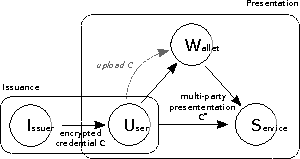
\includegraphics[width=0.6\linewidth]{eABC-System.pdf}
\caption{Overview of an EABC system and its two main protocols.} 
\label{f:overview}
\end{figure} 
\fi
\emph{issuers}, \emph{users}, \emph{services}, and the central \emph{wallet}.
%An issuer is an authority who issues attribute-based credentials in encrypted form to a user, thereby the owner  of such credentials who wish to prove certain attributes to a service, the relying party, while delegating the disclosure process to th \emph{wallet}, a (typically cloud-based) identity provider. 
Each user $U$ holds an \emph{identity key} $sk_U$ proving her identity and which is securely stored on her trusted device (e.g., a smart card or TPM).
$U$ engages in an \emph{issuance protocol} with an issuer $I$ to receive an encrypted credential $C$ on certain attributes only readable to her such that $C$ is bound to her identity key $sk_U$.
$U$ further owns an %anonymous (or pseudonymous\footnote{How a user authenticates to the wallet, and to what extent she needs to identify when setting up her account, is outside the scope of our protocols.}
account managed by the wallet $W$, a typically cloud-based identity provider, to which she uploads all of her encrypted credentials $C$ while not providing it the encryption keys $k(C)$.
At any time later, when $U$ wants to access a service $S$ she is asked to attest some of her attributes. 
To convince $S$ of the requested attributes without revealing any further testified information, $U$ chooses one (or several) of her credentials from her account, selects a subset of attributes contained therein, and instructs $W$ to engage in a \emph{presentation protocol} with $S$, which serves the latter re-encryptions of the requested attributes together with a proof of validity. 
In this protocol, the wallet $W$ undertakes (almost) all costly operations while reducing $U$'s effort to a possible minimum, requiring her only to supply the re-encryption keys for the selected attributes, and a proof of her consent (via her $sk_U$) to the presentation process.
This last proof is also how the overall model of EABCs differs from that in~\cite{towardsEABC}, where no computation is required on the user's side at all;
however, as discussed earlier, we believe this is needed for a realistic attacker scenario, as otherwise the wallet could arbitrarily impersonate the user towards any service provider that the user ever signed up for.



\subsection{Formal Definition}
\label{s:EABCsyntax}

An EABC system with attribute space $\mathbb A$ is built on a structure-preserving blind signature scheme $\BSIG$ in the sense of Section \ref{s:blindAGHO}, an anonymous re-randomizable proxy re-encryption scheme $\PRE$ (cf. Section \ref{s:PRE}) which acts on the  message space of $\BSIG$, and two zero-knowledge proof systems to which we both refer as $\ZKP$ without causing confusion.
Formally, an EABC system
\[
\mathsf{EABC}=(\param, \gen_{I}, \gen_{U}, \issuer, \user_I, \user_P, \wallet, \service)
\] 
consists of the ($\ppt$) algorithms $\param$, $\gen_{I}$, and $\gen_{U}$ for setup and key generation, and the interactive ($\ppt$) algorithms $ \issuer$, $\user_I$, $\user_P$, $\wallet$, $\service$ which are the components of the issuance and presentation protocol described below. 
Given the security parameter $\lambda$, $\param\left(\lambda\right)$ generates the system parameters $sp$.
These are comprised of the parameters for $\BSIG$, $\PRE$, and a common reference string for $\ZKP$.
Every user $U$ holds a PRE secret-public key pair $(sk_U,pk_U)$ generated by $\gen_{U}(sp)=\gen_{PRE}(sp)$, her \emph{identity key}, which is used to generate her certificate pseudonyms.
On demand, a user repeatedly queries $\gen_U(sp)$ to generate the encryption keys $k(C)$ of her credentials. 
Each issuer $I$ is holder of a key pair for the blind signature scheme $(sk_I,vk_I)\leftarrow\gen_I(sp)$, $\gen_{I}=\gen_{BSIG}$, where $sk_I$ denotes the secret signing key and $vk_I$ its public verification key.
Note that, unlike in \cite{towardsEABC}  a service has no permanent key material for the proxy re-encryption scheme.
Its PRE key will be an ephemeral one-time key, one for each presentation.
Both the issuance and the presentation protocol run over server-side authenticated, integrity protected and confidential connections (associated with some random session identifier $sid$) and are as follows.
\begin{description}
\item[Issuance.]
The issuance protocol
\[
\big\langle\user_I\left(sid, sk_U, A, vk_I\right), \issuer\left(sid,  A, sk_I [, pk_U]\right)\big\rangle
\]
is performed between a user $U$ with identity keys $(sk_U,pk_U)$ and an issuer $I$ with signature key pair $(sk_I,vk_I)$ who is the supplier of the random session identifier $sid$.
Both user and issuer agreed on the unencrypted content, the attributes $A=(a_i)_{i=1}^l\in \mathbb A^l$ beforehand.
Depending on the type of issuance, it might be mandatory that $U$ authenticates with its identity key, hence we leave it optional whether $pk_U$ is supplied to $I$ or not, denoted by $[, pk_U]$.
If successful, the protocol outputs to $U$ an encrypted attribute-based credential $(C,vk_I)$ together with it's (secret) key material $sk=sk(C)$, the latter of which $U$ keeps on her device (and  never provides it to a third party).
In all other cases, the user receives $\bot$.

\item[Presentation.]
The presentation protocol  is a three party protocol
\begin{multline*}
\Big\langle\user_P\left(sid, sk_U,sk(C) , D\right), 
\wallet\left(sid, C,D, vk_I\right), \service\left(sid, D, vk_I\right)\Big\rangle
\end{multline*}
and involves a user $U$ with identity key $sk_U$, the wallet $W$ which hosts $U$'s credential $(C,vk_I)$, and a service $S$, who provides the random session identifier $sid$.
As before, $sk(C)$ is the user's secret key material for $C$.
%Depending on the attributes  required by the service, 
The user decides the attributes in $C$ to be disclosed to $S$ beforehand, associated with some index subset $D\subseteq\{1,\ldots,l\}$.
At the end of the protocol the service receives a \emph{presentation} $C^*$ of $C$, which is comprised of the requested attributes, re-encrypted to a random one-time key $sk'$ of $S$, together with a proof of validity.
%This proof is comprised of two linked zero-knowledge proofs, one proving authenticity of the disclosed attributes, and another one proving the active involvment of the owner of the credential in the presentation session.
The service verifies the proof by help of the issuer's public key $vk_I$. 
If valid, the service accepts and decrypts the attributes using $sk'$.
Otherwise it rejects and outputs $\bot$ to both $U$ and $W$.
\end{description}



%\footnotetext{The general case of presenting multiple credentials is discussed in Section \ref{}} 





\subsection{EABC Security Notions}
\label{s:EABCsecurity}

We widen the adversary model from \cite{towardsEABC} to a setting which does not impose any trust assumption on the wallet.
An attacker who controls several players of the EABC system, i.e. the central wallet, some of its users, service providers and issuers, should not be able to compromise the system in a more than obvious manner.
That is, the adversary should not be able to 
\begin{enumerate}
\item
efficiently generate valid presentations which do not match any of the adversary's credentials (\emph{unforgeability}), 
\item
alter the statement of a presentation successfully without knowledge of the user (\emph{non-deceivability}),  
\item
learn anything from the encrypted credentials besides the information disclosed under full control of the owner (\emph{privacy}), and 
\item
distinguish presentations with the same disclosed content when the underlying encrypted credentials are not known to the adversary (\emph{unlinkability}).
\end{enumerate} 
\ifCANS
\else
We note that unforgeability of EABC covers impersonation attacks against honest users, but not a malicious wallet trying to manipulate of the outcome of an honest user's presentation session (within the set of her attributes),  i.e. non-decevability.
Furthermore, since now the adversary takes the position of the wallet as well as a service, we are confronted with two notions of unlinkability:
the untraceability of encrypted credentials back to it's issuance session (covered by privacy), and the indistinguishability of presentations with the same disclosed content (unlinkability).
\fi

All security notions are given in a game-based manner, and we assume server-authenticated, confidential and integrity protected connections between the protocol participants.%, we note that this assumption (which is quite usual from the practical point of view)  may be relaxed for some of the connections (c.f. Remark \ref{rem:rekey}).




\subsubsection{Unforgeability for EABC}
\label{s:EABCunforgeability}
 
The \emph{unforgeability experiment}  paraphrases a malicous wallet and (adaptively many) malicious users,
who altogether try to trick an honest service into accepting a presentation which does not match any of the adversary's queries to an honest issuer.
The experiment manages a  list $L$ which records the key material of all honest system participants during the entire lifetime of the system, i.e. the honest user's identity keys $(pk_U,sk_U)$ and honest issuer keys $(vk_I,sk_I)$.
The list $L$ is also used to log all honest user's credentials $(C, vk_I, sk_U, sk(C))$ under a unique handle $h$.

\emph{
At any time the adversary $\adv$ is given access to all public information contained in $L$, i.e. the public keys $pk_U$, $vk_I$ and the  handles $h$, and as wallet $W^*$ it may retrieve the encrypted credentials $(C, vk_I)$ of every handle $h$ contained in $L$.
}

Besides $L$, the experiment maintains another list $Q_\adv$ used for logging all adversaries queries  to honest issuers of the system. 
At first, the experiment initializes the system by running $sp\leftarrow\param(\lambda)$, setting $L=\emptyset$, $Q_\adv=\emptyset$, and returns $sp$ to the adversary $\adv$.
The adversary may then generate and control adaptively many (malicious) players, and interact with the honest ones by use of the following oracles:
\begin{description}
%\item[Identity generator {$\mathsf{GenID}[id, role, \{key material\}]$}]
%This oracle generates a new system player of role $user/issuer/service$, provided that the identifier $id$ is not list in $L$.
%If the public key material contains a public key $pk$ which is consistent with the queried role, then the oracle simply adds $(id,pk)$ to $L$. (This corresponds to the creation of an adversary-controlled player.)
%If no key material is supplied, then the oracle calls the corresponding key generator $\gen_U$, $\gen_I$ or $\gen_S$ to produce a long-term key pair $(sk,pk)$, and adds both $id$ and $sk$ to $L$.
%(This reflects the creation of honest players).
%\item[Public Key oracle {$\mathsf{PK}[id]$}.]
%This oracle gives the adversary access to the public key of an honest player listed in $L$.

\item[Issuer oracle {$\mathsf{I}(vk_I, A ~[, pk_U^*])$}.]
This oracle, on input an issuer's $vk_I$, attributes $A=(a_i)_i$, and optionally a public identity key $pk_U^*$, provides the adversary a (stateful) interface to an honest issuer's $\issuer(A, sk_I ~[, pk_U^*])$ in the issuance protocol, provided that $vk_I$ is listed in $L$.
If not, then the oracle generates a fresh pair of issuer keys $(sk_I, vk_I)\leftarrow \gen_I(sp)$, adds it to $L$, and returns  $vk_I$ to the caller $\adv$.
Whenever the protocol execution is successful from the issuer's point of view, the oracle adds $(vk_I, (a_i)_i ~[, pk_U^*])$ to $Q_\adv$. 

\item[User-issuance oracle {$\mathsf{U}_I(pk_U, A, vk_I^*)$}.]
This oracle provides the interface to $\user_I(sk_U, A, vk_I^*)$ of an honest user in an adversarily triggered issuance session.
If $vk_I^*$ belongs to an honest issuer (being listed in $L$) the oracle aborts.
As above, if $pk_U$ is not in $L$, the oracle adds fresh $(sk_U,pk_U)\leftarrow\gen_U(pp)$ to $L$, and informs adversary about the new $pk_U$. 
Whenever the session yields a valid credential $C$ for the user, the oracle adds $(C, vk_I^*, sk_U, sk(C))$ together with a fresh handle $h$ to $L$, and outputs $(h, C,vk_I^*)$ to the adversary.

\item[Issuance oracle {$\mathsf{UI}(pk_U, A, vk_I)$}.]
This oracle perfoms a full issuance session between an honest user $pk_U$ and an honest issuer $vk_I$ on the attributes $A$, logs the resulting credential $(C, vk_I, sk_U,$  $sk(C))$  in $L$ and outputs its handle $h$ and the protocol transcript to the caller.
Again, if either $pk_U$ or $vk_I$ are not in $L$ the oracle generates the required identities, adds them to $L$ and returns their new public keys before running the issuance.


\item[User-presentation oracle {$\mathsf{U}_P(h,D)$}.]
The user-presentation oracle initiates a presentation session for an existing handle $h$, and provides both interfaces of  $\user_P(sk_U,sk(C),D)$,where $(sk_U, sk(C))$ belong to $h$,  to the caller.
If the handle $h$ is not listed in $L$, the oracle aborts.
\end{description}
%(Note that there is no need for a separate honest service oracle, since a service keeps no permanent secrets.)
Eventually the adversary $\adv$ runs a presentation session claiming credentials of some honest, but adversarily chosen $vk_I$.
The experiment is successful if $\adv$ manages to make $\service[vk_I]$ accept the presentation but the disclosed attributes $o_S^*= (a_i^*)_{i\in D^*}$ do not correspond to any of the adversary's credentials issued by $vk_I$, which we denote by $o_S^* \notin Q_\adv|_{D^*}$.
% das ist etwas subtil hier, bei angreifergesteuerten Usern wird die Klasse all dieser betrachtet. 
%nor to any  $iid$-issued credential of the honest $uid$ (if the presentation was done for the honest $uid$).
\begin{definition}
\label{def:EABCunforgeability}
An EABC system $\mathsf{EABC}$ is \emph{unforgeable}, if for any $\ppt$ adversary $\adv$ the success probability  in the following experiment is bounded by a negligible function in $\lambda$.
\begin{center}
\fbox{
\procedure{Unforgeability Experiment $\ExpForge(\lambda)$}{
pp \leftarrow \param(\lambda); L = \emptyset; Q_\adv = \emptyset;
\\
(vk_I, st) \leftarrow \mathsf \adv(pp),
\text{ with $vk_I$ listed in $L$}
\\
\langle o_U^*, o_S^*\rangle \leftarrow \big\langle \adv(st), \service(vk_I,D) \big\rangle
\\
\pcif o_U^*\neq \bot \:\wedge\: o_S^*  \notin Q_\adv|_{D^*} ~\pcreturn \text{success}
~\pcelse \pcreturn{\text{failed}}
 }
 }
 \end{center}
In this experiment, $\adv=\adv^{\mathsf{I},\mathsf{U}_I, \mathsf{UI},\mathsf{U}_P}$ has access to the above defined (interactive) oracles, $o_U^*$ denotes the serivce's verdict (ouput to the user-side), and $o_S^*$ are the disclosed attributes $(a_i^*)_{i\in D^{*}}$ (output on the service-side). 
\end{definition}



\subsubsection{Non-Deceivability of Honest Users}
\label{s:EABCnondeceivability}

\emph{Non-deceivability}  (of honest users) is the infeasability of successfully altering the presentation goal without being exposed to the honest user.
Note that this property is not automatically covered by Definition \ref{def:EABCunforgeability}, since such a change of goal might be just between two $vk_I$-credentials of one and the same user.
We formulate this property by means of the \emph{non-deceivability experiment}, which is almost identical to the unforgeability experiment, except that in the last step the adversary $\adv$ opens a presentation session on behalf of an \emph{honest} user for a credential $C$ and index set $D$ chosen by the adversary.

\begin{definition}
\label{def:EABCnondeceivability}
An EABC system $\mathsf{EABC}$ is \emph{non-deceivable towards a user}, if for any $\ppt$ adversary $\adv$ the success probability  in the following experiment is bounded by a negligible function in $\lambda$.
\begin{center}
\fbox{
\procedure{Non-Deceivability Experiment $\ExpDecv(\lambda)$}{
pp \leftarrow \param(\lambda); L = \emptyset;
\\
(h, D, st) \leftarrow \mathsf \adv(pp), 
\text{ such that $h$ is listed in $L$}
\\
\text{Let $C$, $vk_I$, $sk_U$, $sk(C)$, and $(a_i)_i$ belong to $h$}; 
\\
\langle o_U^*, o_S^*\rangle \leftarrow \big\langle \user_P(sk_U,sk(C), D),\adv(st), \service(D,vk_I) \big\rangle
%\\
%(o_U^*, o_S^*) \leftarrow \left\langle \user_P[sk_U, sk(C), D], \adv^{\mathsf{I}, \mathsf{U}_I, \mathsf{U}_P, \mathsf{S}}(st), \service[vk_I] \right\rangle
\\
\pcif o_U^*\neq \bot \wedge  o_S^*  \neq (a_i)_{i\in D}~\pcreturn \text{success}~\pcelse \pcreturn\text{failed}
 }
 }
 \end{center}
As in Defintion \ref{def:EABCunforgeability}, $\adv=  \adv^{\mathsf{I},\mathsf{U}_I, \mathsf{UI},\mathsf{U}_P}$ has access to the  oracles  described in Section \ref{s:EABCunforgeability}, $o_U^*$ denotes the serivce's verdict (ouput to the user-side), and $o_S^*$ are the disclosed attributes $(a_i^*)_{i\in D^*}$ (output on the service-side). 
\end{definition}

%Note that non-deceivability covers the infeasability for the adversary to entirely replace the user by another identity, yet yielding a valid presentation, or to generate a presentation which does not match any of the 





\subsubsection{Privacy for EABC}
\label{s:EABCprivacy}
%

\ifCANS
\else
Privacy for EABC systems, as understood by \cite{towardsEABC} is the indistinguishability of encrypted credentials $(C,vk_I)$ under chosen message attack. 
Allowing wallet-service collusions under which the attacker may get access to disclosed attributes, privacy needs to embrace \emph{untraceability}, i.e. the infeasability of linking  a presentation of an encrypted credential with its  issuance session. 
%%In our adversary model we allow the wallet $W^*$ to collude with an issuer $I^*$ and a service $S^*$, and aim at all three together being not able to deduce any information from a credential, not even its owner's public identity key.
We capture both properties by a single indistinguishability experiment  $\ExpPriv$, which states that nothing more can be learned from a credential $(C,vk_I)$ (not even its owner $pk_U$) than what has been disclosed.
\fi

The adversary's environment in  $\ExpPriv$  is as in the unforgeability experiment from Section \ref{s:EABCunforgeability}.
That is, the experiment maintains a list $L$ for the public and secret data of all honest participants, and 
the adversary is given access to the same honest participant oracles $\mathsf{I}$, $\mathsf{U}_I$, $\mathsf{UI}$, $\mathsf{U}_P$.
First, the experiment generates the system parameters $pp$ and a (random) subset $D\subseteq\{1,\ldots,n\}$, and lets the adversary choose one of its issuance keys $vk_I^*$, two honest (not necessarily different) user identities $pk_{U_1}$, $pk_{U_2}$ and their queries $A_0$, $A_0$ being compliant on $D$, i.e. $A_1|_D=A_2|_D =(a_i)_{i\in D}$.
Then the experiment performs issuance sessions with $vk_I^*$ on $A_0$ and $A_1$ (but does not log the resulting credentials $C_0$ and $C_1$ in the list $L$).
It chooses a random bit $b$, tells the adversary $C_b$ and lets $\adv$ play the wallet and the service in a final presentation session for $C_b$, from which it tries  to guess the random bit $b$. 

\begin{definition}
\label{def:EABCprivacy}
An EABC system $\mathsf{EABC}$ satisfies \emph{privacy}, if for any $\ppt$ adversary $\adv$ the advantage $\left|\prob{
\ExpPriv(\lambda) = \text{success}
} - \frac{1}{2}\right|$  in the following experiment is bounded by a negligible function in $\lambda$.
\begin{center}
\fbox{
\procedure{Indistinguishability Experiment $\ExpPriv(\lambda)$}{
pp \leftarrow \param(\lambda); L = \emptyset; D\sample 2^{\{1,\ldots, l_{max}\}};
\\
(st, vk_I^*, (pk_{U_0}, A_0),(pk_{U_1}, A_1)) \leftarrow \mathsf \adv(pp), 
\\\pcind
\text{with $A_0|_D=A_1|_D$ and $pk_{U_0}$, $pk_{U_1}$ listed in $L$}
\\
\langle (C_i, sk(C_i)), st \rangle \leftarrow \left\langle \user_I(sk_{U_i},A_i,vk_I^*),\adv(st) \right\rangle,
i\in\{0,1\}
\\
b\sample \{0,1\},
\\
b^*\leftarrow \left\langle \user_P(sk_{U_b}, sk(C_b), D, vk_I^*), \adv(st,C_b) \right\rangle
%\\
%(o_U^*, o_S^*) \leftarrow \left\langle \user_P[sk_U, sk(C), D], \adv^{\mathsf{I}, \mathsf{U}_I, \mathsf{U}_P, \mathsf{S}}(st), \service[vk_I] \right\rangle
\\
%b^* \leftarrow
% \adv^{\mathsf{Pres}_b}(st, C_b); 
\pcif{b^*=b}~\pcreturn{\text{success}}~\pcelse \pcreturn{\text{failed}}
 }
 }
 \end{center}
Again, the adversary $\adv= \adv^{\mathsf{I},\mathsf{U}_I, \mathsf{UI},\mathsf{U}_P}$ is given access to  the oracles as described in Section \ref{s:EABCunforgeability}.
\end{definition}

%Note that the experiment's random choice of the subset $D$ is to cover all cases of disclosure extents. 
%Specifically, for $D=\emptyset$ it reflects CPA-security and anonymity of the encrypted credentials.


\subsubsection{Unlinkability of Presentations}
\label{s:EABCunlinkability}

Unlinkability of presentations is the infeasability for a malicious service to link any two presentation sessions with 
the user or the credentials hidden behind the presentation.
Here, the service may collude with issuers (in practice both can be even one and the same entity), but in contrast to the above experiments, the wallet $W$ is assumed to be honest.
%Note that such property is not covered by Defintion \ref{def:EABCprivacy}.
We express this property by means of the \emph{unlinkability experiment}  which is similar $\ExpPriv$ from Section \ref{s:EABCprivacy}, but the adversary is not given access to  the $\mathsf{U}_P$ oracle, and it is forbidden to retrieve any credential $C$ from $L$.
In return it is given access to the following honest wallet oracles:

\begin{description}
\item[Wallet oracle {$\mathsf{W}(h,D)$}]
This oracle provides the interfaces to an honest wallet's $\wallet(C,D,vk_I)$, where  $C$ and $vk_I$ belong to the handle $h$ listed in $L$.
If the handle does not exist, the oracle aborts.

\item[User-wallet oracle {$\mathsf{UW}(h,D)$}]
This oracle, on input the handle $h$ and index subset $D$, 
looks up the corresponding credential $C$ and key material $sk_U$, $sk=sk(C)$ in $L$ and provides the caller the interfaces to the presentation session $\langle \user_P(sk_U, sk(C), vk_I), \wallet(C,D,vk_I), ~.~\rangle$.
As above, if the handle does not exist the oracle aborts.
\end{description}

%The experiment in our definition of unlinkability is almost identical to Defintion \ref{def:EABCprivacy}, with the difference t

\begin{definition}
\label{def:EABCunlinkability}
\footnote{The present definition patches a lapse in the formal definition of the unlinkability experiment as given in \cite[Definition 7]{DBLP:conf/cans/HabockK19}, which mistakenly refers to guessing the issuance session behind the presented credentials.
}
An EABC system $\mathsf{EABC}$ is \emph{unlinkable}, if for any $\ppt$ adversary $\adv$   the advantage
$
\left|\prob{
\ExpUnlink(\lambda) = \text{success}
} - \frac{1}{2}\right|
$
in the following experiment is bounded by a negligible function in $\lambda$.
\begin{center}
\fbox{
\procedure{Unlinbkability Experiment $\ExpUnlink(\lambda)$}{
pp \leftarrow \param(\lambda); L = \emptyset;
\\
(st, vk_I^*, h_0, h_1, D, (a_i)_{i\in D}) \leftarrow \mathsf \adv(pp), 
\\
\pcind \text{with both $C_i=C(h_i)$ as valid $vk_I^*$-credentials  encoding $(a_i)_{i\in D}$}
\\
\text{Let $(pk_{U_i}, C_i)$ and $sk(C_i)$ belong to handle $h_i$.}
\\
b\sample \{0,1\};
\\
b^* \leftarrow  \left\langle \user_I(sk_{U_b},sk(C_b),D), \wallet(C_b,D,vk_I^*), \adv(st, (pk_{U_0},C_0),(pk_{U_1}, C_1)\right\rangle
\\
\pcif{b^*=b}~\pcreturn\text{success}
\pcind\pcelse \pcreturn\text{failed}
 }
 }
 \end{center}
In the experiment the adversary $\adv=\adv^\mathsf{I,U_1, UI, W, UW}$ is given access to all the honest-participant oracles from Section \ref{s:EABCunforgeability}, and the above defined honest wallet oracle $\mathsf{W}$ and $\mathsf{UW}$. 
Besides $C_0$ and $C_1$ it is not given access to any credentials listed in $L$.
\end{definition}


\section{Instantiating EABCs}
\label{s:EABCinstantiation}

%
% This variant uses Pedersen commitments for the linearization of the zero knowlegde proofs
%
We instantiate  $\mathsf{EABC}=(\param, \gen_{I}, \gen_{U}, \mathsf{User}_I,\issuer, \mathsf{User}_P,$ $\wallet, \service)$ using 
%\begin{itemize}
%\item 
the structure-preserving  blind signature scheme $\BSIG=\BSIG_{AGHO}$ from Section \ref{s:blindAGHO}, 
%\item
the anonymous re-randomizable proxy re-encryption scheme $\PRE=\PRE_{BBS}$ by Blaze, Bleumer, and Strauss (BBS, cf. Section \ref{s:PRE}), 
%\end{itemize}
%Pedersen's commitment scheme $\COM=\COM_{PED}$ for committing PRE secret keys, 
and two non-interactive zero-knowledge proof systems  (cf. Section \ref{s:ZKP}), one of which is simulation extractable.
For notational convenience, we shall refer to both as $\nizk$ without causing confusion.
%We stress not to confuse $\COM$ with the commitment scheme used for the restrictive blind signature scheme, which is solely based on the PRE encryption as explained below.  



\subsection{System Parameters and Key Generation}
Given the security parameter $\lambda$, a trusted\footnote{
In practice, the generation of the system parameters can be realized using multi-party techniques.
}
third party generates  the system parameters by $sp\leftarrow\param(\lambda)$,
which internally queries $\param_{BSIG}$ and  $\param_{PRE}$ %$\param_{COM}$, 
in such a way that the message space for $\BSIG$ and  the ciphertext space of $\PRE$ is the same group $\mathbb G$ of prime order $q$.
%, and the commitment space of $\COM$ 
Furthermore, it uses $\gen_{ZKP}$ to set up a common reference string for the $\nizk$.
%(The latter can be easily instantiated in the random oracle by a hash function )
%, and furthermore that $\Z_q$ can be efficiently embedded into the message space $E:\Z_q\longrightarrow\mathcal M_\mathsf{ENC}$ of $\mathsf{ENC}$.
%(This can be realized with help of an external group generator.)
Specifically, the system parameters are 
\[
sp=\left(L, \mathbb G,\mathbb H,\mathbb T, q, e, G, H, g, crs\right),
\] 
whereas $L$ is the maximum number of attributes allowed in a credential,
$\mathbb G$, $\mathbb H$, $\mathbb T$ are the AGHO pairing groups of prime order $q$, with bilinear mapping $e: \mathbb G\times \mathbb H\longrightarrow \mathbb T$  and respective generators $G$, $H$, and $e(G,H)$, $g\in \mathbb G$ is the generator for the BBS encryption scheme, 
%and $g_1, g_2\in \mathbb G$ are the generators for the  BBS scheme and the Pedersen commitments, 
and $crs$ is the common reference string for the NIZK proof systems.
%The parameters of our key establishment scheme, $pp_{AKE}$, consists of a Diffie-Hellman group $G_{AKE}$ with generator $g_{AKE}$ and a hash function $\hash:G_{AKE}\rightarrow\Z_q$ with an output distribution  statistically close to the uniform distribution on $\Z_q$.
We further assume that all attributes $a\in\mathbb A$ are represented by group elements from $\mathbb G$.
%\footnotetext{
%There are four NIZK proof systems involved.
%For simplicity we nevertheless gather their CRSs into a single one, which shall cause no confusion for the reader.  
%}

An issuer $I$'s signing key generated by $\gen_I(sp)=\gen_{BSIG}(sp)$ consists of the AGHO keys $sk_I=(v, (w_i)_{i=1}^l, z)$ and $vk_I=(V,(W_i)_{i=1}^l, Z)$, where $l\leq L$, 
and  a user's identity key consists of the BBS keys $(sk_U,pk_U)$ generated by $\gen_U(sp)=\gen_{PRE}(sp)$.
%On demand, $U$ queries $\gen_{PRE}$ as often as necessary to generate further key material, the \emph{attribute keys} $(sk_i,pk_i)_{i=1}^l$, for a credential.
%A service $S$ generates its long term key for its authenticated channel establishment $(\sk_S,\pk_S)\leftarrow\gen_{AKE}$.  

%Note that, in contrast to \cite{towardsEABC} a service $S$ does not hold a long-term key (unless one wants to instantiate a variant of the $\rekey$ protocol below which uses the wallet $W$ as a proxy, cf. Section \ref{s:protocols}).

%\textcolor{red}{Dieser Absatz ist später teilweise nicht mehr notwendig}
%Besides involving all three parties, the user $U$, the wallet $W$ and the service $S$ in the presentation protocol, there are two major differences to the instantiation from \cite{towardsEABC}.
%Firstly, we use the blinded variant for the AGHO signature as described by Protocol \ref{prot:blindAGHO} to achieve the unlinkability of issued credentials  to their issuance session.
%Secondly, we use separate BBS keys for attribute encryption (\emph{attribute keys}), and random one-time re-encryption keys for each presentation session.
%We further optimize the presentation proof by directly mapping  the re-encryptions for $S$ into the verification equation of the AGHO signature.
%One the one hand, this decreases the number of equations of the proof and reduces the amount of data to be communicated to the service.
%\textcolor{red}{
%Secondly, and much more important, this  allows us to work without the security notion of \emph{anonymous} PRE as in \cite{towardsEABC}.
%}


\subsection{Issuance}
\label{s:issuance}



%An enrypted credential as issued by Protocol \ref{prot:issuance} will be of the form 
%\[
%c = (c_{i,0}, c_{i,1},c_{i,2})_{i=0}^l = (g^{sk_i}, g^{r_i}, g^{r_i\cdot sk_i} \cdot a_i)_{i=0}^l, 
%\]
%with $a_i \in\mathcal A$ and $a_0=1$, and an AGHO signature $\sigma=(R,S,T)$ on $c$.
%The issuance protocol essentially is the restrictive blind AGHO scheme for the language $\mathcal L$
%of all such $c=(c_{i,0},c_{i,1},c_{i,2})_i$ with witness $s=(sk_i)_{i=0}^l$ and 
%restriction function $f(y,(c,s)) = c_{i,1}^{-sk_i}\cdot c_{i,2} \cdot y^{-1}$ for any given attributes $y=(a_i)_{i=0}^l$ with $a_0=1$.
The issuance protocol is the restrictive blind AGHO signature (Definition \ref{prot:blindAGHO}) based on the commitment 
\[
\comm(sk_U,(a_i)_i) = (c_0, (pk_i,c_i)_i), %= (\enc_{BBS}(pk_U, 1), (pk_i, \enc_{BBS}(pk_i, a_i))_i)
\]
which embodies the encrypted certificate to be signed, being comprised by  $U$'s \emph{certificate pseudonym} $c_0 =  \enc_{BBS}(pk_U, 1)$, and the \textit{attribute encryptions} $c_i  =\enc_{BBS}(pk_i, a_i)$ with respect to fresh proxy re-encryption keys $(pk_i)_i$.
% altogether as commitment for $x= (sk_U, (a_i)_i)$.
%Note that $com$ uniquely determines $x$ and its opening $w$ where $w=(sk_U, (sk_i)_i)$ consists of the secret  PRE keys belonging to $pk_U$ and $(pk_i)$.
%Given IND-CPA security and anonymity of the BBS scheme (both of which follow from the DDH assumption on $\mathbb G$) this way to commit on $pk_U$ and $(a_i)_i$ is perfectly binding and computationally hiding.
Although authentication of $U$ is outside the scope of the blind AGHO scheme, %and could be as well transferred to a separate procedure in the setting of EABC,   
we nevertheless integrate it into the issuance protocol by extending the wellformedness proof of the restrictive scheme by a proof of knowing the secret key belonging to $pk_U$.
%Versions where the user is allowed to stay anonymous or pseudonymous towards the issuer are discussed in Remark \ref{rem:issuance}. 
The protocol runs over a server-authenticated, confidential and integrity protected channel.

\begin{definition}[Issuance Protocol]
\label{prot:issuance}
%The issuance protocol %of encrypted attribute-based credentials 
$\big\langle \user_I(sid, sk_U, (a_i)_{i=1}^l, vk_I), \issuer(sid, {pk_U}$, $(a_i)_{i=1}^l, sk_I)\big\rangle$
is a protocol between a user $U$ with identity key $(sk_U,pk_U)$ and an issuer $I$ with AGHO keys $(sk_I,vk_I)$. %who supplied the random session identifier $sid$.
Both user and issuer agreed on the unencrypted content, the attributes $A = (a_i)_{i=1}^l\in \mathbb A^l$, beforehand.
%We further assume that the user $U$ is demanded by $I$ to supply her identity $\pk_U$, and refer to Remark \ref{rem:issuance} for the case of anonymous issuance.
\begin{enumerate}
\item
$U$ computes $com = \left(c_0, (pk_i,c_i)_{i=1}^l\right)$  by generating a fresh  pseudonym $c_0 = (c_{0,1},c_{0,2}) = \enc_{BBS}(pk_U, 1)$ and  attribute encryptions $c_i = (c_{i,1}, c_{i,2}) = \enc_{BBS}(pk_i, a_i)$ using a fresh set of attribute keys $(sk_i,pk_i)\leftarrow\gen_{BBS}(sp)$, $1\leq i \leq l$.
For notational convenience we write $m=(m_{i,j}) = ( pk_i,c_{i,1},c_{i,2})_{i=0}^l $ for  $com$, where we set $(sk_0,pk_0)=(sk_U,1)$ and $a_0=1$.

\item
With the above described commitment scheme, $U$ engages the restrictive blind signing session with $I$ (Definition \ref{prot:blindAGHO}) to receive an \emph{encrypted credential} 
\begin{equation*}
\label{e:credential}
C= \left\{\left(c_0,  \left(pk_i, c_i\right)_{i=1}^l\right), \sigma = (R,S,T)\right\},
\end{equation*}
with $\sigma$ being a valid AGHO signature by $I$ on $com$, and with $(sk_i)_{i=0}^l$ as the opening of $com$.
Demanding additional authentication of the user $U$ by means of her identity key $sk_U$, 
 the zero-knowledge proof $\pi_U$ as described in Definition \ref{prot:blindAGHO}, is explicitly described by
\begin{align*}
\pi_U = \nizk\bigg[\big(\eta, \varphi_1, \varphi_2, (\kappa_i,\lambda_i&)_{i=0}^l\big) :
g^{\kappa_0}=pk_U  
\\
&\wedge~ G_1^\eta = G  ~\wedge~  G^{\varphi_1}= G_2 ~\wedge~ G_1^{\varphi_2} = G_3
\\&
\bigwedge_{i=0}^l  
G_1^{\lambda_i} = G^{\kappa_i} \wedge
\overline{m}_{i,0}\cdot \overline P_{i,0}^{\eta} = g^{\kappa_i} 
\wedge
 \overline m_{i,2}\cdot \overline P_{i,2}^{\eta}  = \overline m_{i,1}^{\kappa_i} \cdot \overline P_{i,1}^{\lambda_i} \cdot a_i   
\bigg],
\end{align*}
which is bound to the unique session identifier $sid$.
Here, the user $U$ chooses $(\eta, \varphi_1, \varphi_2) = (\nicefrac{1}{e},f_1,f_2)$, and $(k_i,\lambda_i) = (sk_i, \nicefrac{sk_i}{e})$, $0\leq i\leq l$, as witnesses. 
%After successul completion of Protocol \ref{prot:blindAGHO}, the user $U$ is finally in posession of an encrypted credential 
%\begin{equation}
%\label{e:credential}
%\left(c_0,  \left(pk_i, c_i\right)_{i=1}^l\right), \sigma = (R,S,T),
%\end{equation}
%with $\sigma$ being a valid AGHO signature by $I$ on $c_0$ and $(pk_i, c_i)_{i=1}^l$.
%$U$ keeps $r_0$ and the secret attribute keys $(sk_i)_{i=1}^l$.
\end{enumerate}
%She then sends $(G_1,G_2,G_3)$, $\overline m$, $\overline P$, together with the proof $\pi$ to the issuer.
%sends  $\left(\overline pk_i, \overline c_i\right)_{i=0}^l$, $\overline G_1$, $\overline G_2$, $(\overline h_{i,j})$, and $\pi$ to the issuer.
\end{definition}

\begin{remark}
\label{rem:issuance}
In some situations a user might be allowed to stay anonymous towards the issuer.
In such case the user's public identity $pk_U$ is not part of the commited $x$ and hence not provided to $I$, the term $g^{\kappa_0}=pk_U$ in $\pi_{U}$ is omitted.
In another setting similar to \cite{brands99,idemix} a user might be known to $I$ under a pseudonym $P_U=\enc_{BBS}(pk_U, 1)$ of her. 
Here, $U$ proves to $I$ that the same secret key $sk_U$ is used in both $P_U=(P_{U,1},P_{U,2})$ and the certificate pseudonym, replacing $g^{\kappa_0}=pk_U$ by $c_{0,1}^{\kappa_0} = c_{0,2} ~\land ~ P_{U,1}^{\kappa_0} = P_{U,2}$.
\end{remark}

\subsection{Presentation}

The presentation of a credential $C$, as described in full detail by Definition \ref{prot:presentation}, is essentially based on re-encrypting a re-randomization of $C$ into a selective readable version $\overline C$ for the service $S$, supplemented by two linked zero-knowledge proofs:
%, altogether forming a two-prover zero-knowledge proof:
the computationally costly \emph{presentation proof} $\pi_P$, which is performed by the wallet $W$ and which relates the transformed $\overline C$ to the original $C$ (the latter, including its signature is hidden from $S$),  and  the \emph{ownership proof} $\pi_O$ on the pseudonym of $\overline C$, proving knowledge of the secret identity key belonging to the pseudonym.
%As aforementioned, the active involvement of the owner of the credential, in our case demanded by supplying $\pi_O$, is necessary to impersonation of the user by the wallet.
The first proof is efficiently  instantiated by help of the structure-preservation property of the blind AGHO scheme, the ownership proof supplied by the user is a simple proof of knowledge of a 
 single exponent. 
%In both proofs, ciphertext re-randomization takes a prominent role in assuring the unlinkability of the presentation with the credential $C$ behind it.

%The plot in Protocol \ref{prot:presentation} is as follows:
%First of all, the user $U$ establishes an ephemeral session key $sk'$ with the service $S$, and derives the re-encryption keys $(rk_i)_{i\in D}$ corresponding to selected attributes (by choosing the index set $D\subseteq\{1,\ldots ,l\}$).
%It then re-randomizes the credential's pseudonym $c_0$ (or lets $W$ do it), keeps the used randomness $r$, and sends $S$ a fresh ownership proof $\pi_O$ on the re-randomized pseudonym $\overline c_0$.
%In the second step, $U$ informs the wallet $W$ about the re-encryption keys $(rk_i)_{i\in D}$, $\overline c_0$ and $r$, which then re-randomizes and re-rencrypts the selected attributes to obtain $\overline C$, which is sent to $S$ together with the presentation proof $\pi_P$.
%Eventually, $S$ verifies both the ownership proof $\pi_O$ and $\pi_P$. 
%If valid, it is convinced of the authenticity of $\overline C$ and uses the one-time key $sk'$ to decrypt the corresponding attributes in $\overline C$.


For the sake of readability, we gather the establishment of the service's session keys  and its corresponding transformation information in a separate subprotocol, the $\rekey$ protocol. 
Both Protocols from Defintion \ref{prot:rekey} and  \ref{prot:presentation} run over a server-authenticated, confidential and integrity protected channel, and are associated with the same random session identifier $sid$ supplied by the service.
Furthermore, the non-interactive proofs ($\pi_O$ and $\pi_S$ below) are bound to the context of the presentation, in particular the common public parameters $sid$, $vk_I$ and $D$.

%It's main purpose is to establish random re-encryption keys for the presentation session, which can be realized in various ways, e.g. by letting solely $U$ generate it (and send it confidentially to $S$), or by authenticated DH like protocols which provide forward secrecy.  
%In practice, in order not to reveal its IP address the user will contact $S$ via a proxy,  e.g. the wallet itself, or Tor.

\begin{definition}[$\rekey$ protocol]
\label{prot:rekey}
This protocol between the user $U$
and the service $S$ is  a subprotocol of the presentation protocol from Defintion \ref{prot:presentation}.
\begin{enumerate}
\item
$U$ chooses a random one-time key $sk'\sample\Z_q$, and forwards $sk'$ and $D$ to $S$.

%$U$ chooses random one-time keys for the attributes to be disclosed, i.e $(sk'_i)_{i\in D}$ with $sk_i\sample\Z_q$, and sends $(sk'_i)_{i\in D}$ to $S$.

\item
$U$  re-randomizes\footnotemark her pseudonym $c_0$ by $e\sample \Z_q$, $\overline c_0 = \left(\overline c_{0,1}, \overline c_{0,2}\right) = \left(c_{0,1}^{e}, c_{0,2}^{e}\right)$ and proves to $S$ that she is in posession of its secret key, by supplying a simulation extractable zero-knowledge proof
\[
\pi_O=\nizk\left[ \kappa : \overline c_{0,1}^\kappa = \overline c_{0,2}\right],
\] 
%which is bound to the session identifier $sid$, and in which 
in which she uses $\kappa = sk_U$ as witness.

\item
$S$ verifies $\pi_O$, and if valid it keeps $\overline c_0$ and $sk'$.%, establishes a secure connection with $W$, compute its ephemeral public keys $(pk_i')_{i\in D}$ and forwards them to $W$.
Otherwise, $S$ aborts the protocol.
On the user side, $U$ takes the secret attribute keys $(sk_i)_i$ belonging to $C$ and determines $rk_0'=\nicefrac{1}{e}$ and the re-encryption keys $rk_i' = \nicefrac{sk_i}{sk'}$, $i\in D$.
%\item
%$S$ verifies $\pi_O$, and if valid it $S$ keeps the pseudonym $\overline c_0$ (which it might use as session identifier) and waits to get contacted by $W$.
%Otherwise, $S$ aborts the protocol.
%On the user side, 
\end{enumerate}
\footnotetext{For the sake of efficiency, $U$ might outsource the re-randomization of its pseudonym to the wallet.
}

%\begin{enumerate}
%\item
%$U$ receives a nonce $n_s$ from $S$, generates a random secret key $sk'\sample\Z_q$ for $\PRE_{BBS}$, 
%and sends $ck' = \enc_{ENC}(pk_S,sk'||n_s)$ to $S$.
%\todo{
%we need to guarantee fresheness of $sk'$ to the service provider!% to mitigate replay attacks!
%}
%%and sends it in (for $pk_S$) encrypted form to $S$.
%%by performing an authenticated key exchange with $S$ (using the $\mathsf{AKE}$ scheme).
%%$\langle\user_{AKE}(pp_AKE,pk_S),\service_{AKE}(pp_{AKE}, sk_S) \rangle$ .
%
%\item
%$U$ re-randomizes its credential pseudonym $c_0$ by $r\sample \Z_q$, $\overline c_0 = \left(\overline c_{0,1}, \overline c_{0,2}\right) = \left(c_{0,1}^{r}, c_{0,2}^{r}\right)$ and 
%generates  a zero-knowledge proof  that she knows the secret key for the re-randomized pseudonym, 
%\[
%\pi_O=\ZKP\left[(\kappa) : \overline c_{0,1}^\kappa = \overline c_{0,2}\right],
%\] 
%for which she uses $\kappa = sk_U$ as witness.
%\todo{again, to guarantee freshness it is important that the NIZKP is bound to the session nonce $n_s$ or $sk'$.}
%She then takes the secret attribute keys $(sk_i)_i$ belonging to $C$ and determines $rk_0'=\frac{1}{r}$ and the re-encryption keys $rk_i' = \frac{sk_i}{sk'}$, $i\in D$.
%
%%\item
%%$S$ verifies $\pi_O$, and if valid $S$ keeps the pseudonym $\overline c_0$ (which can be used as session identifier) and waits to get contacted by $W$ (in practice $S$ initiates the communication between $S$ and $W$).
%%Otherwise, $S$ aborts the protocol.
%
%%\item
%%$U$  re-randomizes its credential pseudonym $c_0$ by $r\sample \Z_q$, $\overline c_0 = \left(\overline c_{0,1}, \overline c_{0,2}\right) = \left(c_{0,1}^{r}, c_{0,2}^{r}\right)$ and proves to $S$ in zero-knowledge that she knows the secret key for the re-randomized pseudonym, 
%%\[
%%\pi_O=\ZKP\left[ (\kappa) : \overline c_{0,1}^\kappa = \overline c_{0,2}\right],
%%\] 
%%in which she uses $\kappa = sk_U$ as witness.
%%\item
%%$S$ verifies $\pi_O$, and if valid $S$ keeps the pseudonym $\overline c_0$ (which can be used as session identifier) and waits to get contacted by $W$ (in practice $S$ initiates the communication between $S$ and $W$).
%%Otherwise, $S$ aborts the protocol.
%%On the user side, $U$ takes the secret attribute keys $(sk_i)_i$ belonging to $C$ and determines $rk_0'=\frac{1}{r}$ and the re-encryption keys $rk_i' = \frac{sk_i}{sk'}$, $i\in D$.
%\end{enumerate}
\end{definition}

%\begin{remark}
%\label{rem:rekey}
%%As mentioned before, instead relying on an service-authenticated channel one may directly use any (one-sided) authenticated key establishment scheme between $U$ and $S$ and use as long it satisfies similar mild security properties, e.g. being $SK$-secure in the sense of \cite{AKE:Canetti}. 
%If one wants to avoid direct communcation of the user with an internet-based service $S$ (for transport layer privacy, e.g.) the entire commication between $U$ and $S$ can be implemented using the wallet as a proxy. 
%Such proxy functionality is easily implemented on application layer by using a separate (service-side) authenticated key establishment scheme such as HMQV.
%Demanding explicit communication between $U$ and $S$ is just for the sake of generality, if one wants to replace our one-pass key exchange by another key agreement scheme (with similar security properties).
%In our setting, the session nonce and encrypted one-time key might be sent as well via the wallet as a prox          y. %As mentioned before, any AKE scheme between $U$ and $S$ can be used as long as it satisfies similar security properties.
%\end{remark}


\begin{definition}[Presentation Protocol]
\label{prot:presentation}
The presentation protocol of encrypted attribute-based credentials $\big\langle \user_P(sid, sk_U, (sk_i)_{i\in D}), \wallet(sid, C, D,vk_I), \service(sid, D, vk_I)\big\rangle$ 
is between a user $U$ with identity key $sk_U$ who owns the credential $C$ issued by $I$, the wallet $W$, and the service $S$ (the supplier of the random session identifier $sid$).
Here, $D\subseteq\{1,\ldots,l\}$ denotes the index set of the attributes to be disclosed, and $(sk_i)_{i\in D}$ are $U$'s corresponding attribute keys.
 %of a single credential $C$ and refer to \ref{rem:multishow} to the case of multi-show presentations.
\begin{enumerate}
\item
$U$ performs Protocol  from Definition \ref{prot:rekey} with $S$, and if successful it sends the re-randomized one-time pseudonym $\overline c_0$ together with the re-encryption keys $rk_0'$, $\left(rk'_i\right)_{i\in D}$ and $D$ to $W$.

%\item
%$U$ and $S$ agree on a random one-time private key $sk'$ for $\PRE_{BBS}$ by performing an authenticated key exchange with $S$ (using the $\mathsf{AKE}$ scheme).
%$\langle\user_{AKE}(pp_AKE,pk_S),\service_{AKE}(pp_{AKE}, sk_S) \rangle$ .

%\item
%$U$  re-randomizes its credential pseudonym $c_0$ by $r\sample \Z_q$, $\overline c_0 = \left(\overline c_{0,1}, \overline c_{0,2}\right) = \left(c_{0,1}^{r}, c_{0,2}^{r}\right)$ and 
%generates  a zero-knowledge proof  that she knows the secret key for the re-randomized pseudonym, 
%\[
%\pi_O=\ZKP\left[ \kappa : \overline c_{0,1}^\kappa = \overline c_{0,2}\right],
%\] 
%for which she uses $\kappa = sk_U$ as witness.
%She then takes the secret attribute keys $(sk_i)_i$ belonging to $C$, determines $rk_0'=\frac{1}{r}$ and the re-encryption keys $rk_i' = \frac{sk_i}{sk'}$, $i\in D$, and sends $\overline c_0$, $rk_0'$, $\left(rk'_i\right)_{i\in D}$ and $\pi_O$ to $W$.

\medskip
\item[]{From now on we proceed similar to \cite{towardsEABC}:}
\item
(Randomization and re-encryption) For $i\in D$, the wallet $W$ re-randomizes the ciphertexts $c_i$ to $\overline c_i =  \left(c_{i,1}\cdot g^{f_i}, c_{i,2}\cdot pk_i^{f_i}\right)$, with $f_i\sample\Z_q$. 
All other attributes are randomized inconsistently, by choosing  $v_{i,0}$, $v_{i,1}$, $v_{i,2}\sample\Z_q$ and setting $\overline{pk}_i = pk_i \cdot g^{v_{i,0}}$, $\overline c_i = \left(c_{i,1} \cdot g^{v_{i,1}}, c_{i,2}\cdot g^{v_{i,3}}\right)$ for all $i\not\in D$.
Using the re-encryption keys $\left(rk_i'\right)_{i\in D}$ the wallet translates the attributes belonging to $i\in D$ by $d_i =\reenc_{BBS}\left(rk_i', \overline c_i\right) =\left(\overline c_{i,1}^{rk_i'}, \overline c_{i,2}\right)$.

\item 
(Presentation)
$W$ randomizes $T$ by $\overline T = T^x$, $x\sample\Z_q$, %computes the Pedersen commitments  $k_i = \COM(\nicefrac{1}{rk_i'}, s_i) = g_1^{\nicefrac{1}{rk_i'}}\cdot g_2^{s_i}$, $s_i\sample\Z_q$, for all $i\in D$.
%Being contacted by $S$ and provided with the session identifier $sid$, the
forwards $ \left(d_i \right)_{i\in D}$,  $\left( \overline{pk}_i, \overline c_i\right)_{i \notin D}$, and $\overline T$ to $S$, and provides a wellformedness proof of these elements via
 %   the ciphertexts $ \left(d_i \right)_{i\in D}$ are derived properly by (re-)randomization and re-encryption from a valid credential, %i.e. it derives the proof of wellformedness
\begin{align*}
\pi_P= \nizk\Big[
(P, \Sigma, \xi), \eta,  (\kappa_{i}, \gamma_{i})_{i\in D}, (\nu_{i,0}, \nu_{i,1}, \nu_{i,2})_{i\notin D}
:
\text{\eqref{e:zkpsig1}} \wedge
\text{\eqref{e:zkpsig2}} % ~\land~\bigwedge_{i\in D} \left(\text{\eqref{e:zkpComm2}}\wedge \text{\eqref{e:zkpComm3}}\right)
\Big],
\end{align*}
which is defined by the relations \eqref{e:zkpsig1} and \eqref{e:zkpsig2} below.

%, and which is bound to the session identifier $sid$.
%,\eqref{e:zkpComm2} and \eqref{e:zkpComm3} described below.  
%The proof rephrases


\item
$S$ verifies $\pi_P$ using the verified one-time pseudonym received in Protocol \ref{prot:rekey}.
If valid, it decrypts the attributes  $\left(d_i\right)_{i\in D}$ with its one-time key $sk'$.
(Otherwise $S$ outputs $\bot$).
\end{enumerate}
\end{definition}

\begin{remark}
\label{rem:multishow}
Showing more than one credential is efficiently implemented by merging their ownership proofs to a single $\nizk$ which simultaneously proves knowledge of $sk_U$ on all used pseudonyms, $\nizk \left[ (\kappa) : \bigwedge_{C} \overline  c_{0,1}(C)^\kappa = \overline c_{0,2}(C)\right]$.
\end{remark}


Equation \eqref{e:zkpsig1} and \eqref{e:zkpsig2} mentioned in Protocol \ref{prot:presentation}, state that $(P, \Sigma, \overline T^{\nicefrac{1}{\xi}})$ is a valid signature for a quadratic derivative of the above group elements  $\left(\overline c_{0,1}, \overline c_{0,2}\right)$, $(d_{i,1}, d_{i,2})_{i\in D}$ and $(\overline{pk}_i,\overline c_{i,1},\overline c_{i,2})_{i\not\in D}$, 
i.e.
\begin{multline}
\label{e:zkpsig1}
e(\Sigma, H)\cdot  e(\rho, V) \cdot e(\overline c_{0,1}, W_{0,1})^{\eta} \cdot e(\overline c_{0,2},W_{0,2})^{\eta}\cdot 
\\
\cdot 
\prod_{i\in D} e\left(pk',W_{i,0}\right)^{\kappa_{i}} \cdot e(g, W_{i,1})^{-\gamma_{i}\cdot \kappa_i} \cdot e(pk', W_{i,2})^{-\gamma_i}\cdot
\\
\cdot \prod_{i\not\in D} e\left(g,W_{i,0}\right)^{-\nu_{i,0}} \cdot e(g, W_{i,1})^{-\nu_{i,1}} \cdot e(g, W_{i,2})^{-\nu_{i,2}}\ =
\\ 
= e(G,Z)
\cdot\prod_{i\in D} e(d_{i,1}, W_{i,1})^{-1} \cdot  e(d_{i,2}, W_{i,2})^{-1} \cdot \\
\prod_{i\not\in D}  e(\overline{pk}_i, W_{i,0})^{-1} \cdot   e(\overline c_{i,1}, W_{i,1})^{-1} \cdot  e(\overline c_{i,2}, W_{i,2})^{-1},
\end{multline}
where $V$, $Z$, and $(W_{i,0}, W_{i,1}, W_{i,2})_{i=0}^l$ are the components of the issuers verification key, and
\begin{align}
\label{e:zkpsig2}
e(P, \overline T) \cdot  e(G,H)^{-\xi} &= 1.
\end{align}
%and the other $2\cdot |D|$ equations show that  for  $i \in D$, the signed elements where derived via correct re-encryption and re-randomization, i.e. 
%\begin{align}
%%\label{e:zkpComm1}
%%\overline c_{i,1}^{\delta_{i,0}} &= d_{i,1},
%\label{e:zkpComm2}
%g_1^{\delta_{i,0}}\cdot g_2^{\theta_{i,0}} &= k_i,
%\\
%\label{e:zkpComm3}
%k_i^{\delta_{i,2}} \cdot g_1^{-\delta_{i,1}}\cdot g_2^{-\theta_{i,1}} &= 1,
%\end{align}
%for all $i\in D$.
\ifCANS
Linearization of the quadratic terms in \eqref{e:zkpsig1} is accomplished by standard techniques and given in the full version of the paper.
An honest prover chooses $(P,\Sigma, \xi) = (R,S,x)$, and uses the parameters from step 2 of Protocol \ref{prot:presentation}, i.e.  $\eta = rk_0'$, $\left(\kappa_{i},\gamma_{i}\right) = \left(\nicefrac{1}{rk_i'}, rk_i'\cdot f_{i}\right)$ for $i\in D$, and $\left(\nu_{i,0},\nu_{i,1},\nu_{i,2}\right) = \left(v_{i,0}, v_{i,1}, v_{i,2}\right)$ for all $i\not\in D$.

\else
Linearization of the quadratic terms in \eqref{e:zkpsig1} is accomplished by standard techniques and given in Appendix \ref{s:linearization}.
An honest prover chooses $(P,\Sigma, \xi) = (R,S,x)$, and uses the parameters from step 2 of Protocol \ref{prot:presentation}, i.e.  $\eta = rk_0'$, $\left(\kappa_{i},\gamma_{i}\right) = \left(\nicefrac{1}{rk_i'}, rk_i'\cdot f_{i}\right)$ for $i\in D$, and $\left(\nu_{i,0},\nu_{i,1},\nu_{i,2}\right) = \left(v_{i,0}, v_{i,1}, v_{i,2}\right)$ for all $i\not\in D$.
\fi

%\todo{ist das ueberhaupt interessant? die Proofs sind ohnehin relativ gross}


%We conclude this section with the security statement on our $EABC$ instantiation.
\begin{theorem}
\label{thm:EABC}
Suppose that the AGHO signature scheme is EUF-CMA secure, and that 
the $\nizk$ from Definition \ref{prot:rekey} is simulation extractable.
%, whereas the other one from Defintion \ref{prot:presentation} is extractable.
Then, under the DDH-assumption in $\mathbb G$, 
\begin{enumerate}
\item
\label{thm:EABC:i}
the proxy re-encryption scheme $\PRE_{BBS}$ is PRE-IND-CPA secure, anonymous, and has the ciphertext re-randomization property,
\item
\label{thm:EABC:ii}
the structure-preserving blind signature scheme $\mathsf{BSIG}_{AGHO}$ is unforgeable and has the blinding property,
%\item
%\label{thm:EABC:iii}
%the Pedersen commitment scheme $\COM_{PED}$ is computationally binding and hiding.
\end{enumerate}
hence our EABC system satisfies \emph{unforgeability}, \emph{non-deceivability}, \emph{privacy} and \emph{unlinkability}  in the sense of  Section \ref{s:EABCsecurity}.
%Furthermore, if the AGHO signature scheme is EUF-CMA secure, the EABC scheme fulfills  according to Defintion and .
%If the structure-preserving signature scheme $\BSIG$ satisfies blindness (which $\BSIG_{AGHO}$ does under the DDH-assumption in $\mathbb G$), and the PRE scheme is IND-CPA (satisfied by the BBS scheme under the DDH-assumption in $\mathbb G$), then the EABC system is \emph{private under active adversaries}.
%Furthermore, if $\BSIG$ is unforgeable (which $\BSIG_{AGHO}$ is in the generic group model), and $COM$ is computationally binding commitment scheme (which the Pedersen commitments are under the DL assumption in $\mathbb G$), then the EABC system is unforgable.
\end{theorem}
\ifCANS
The proof of Theorem \ref{thm:EABC} is given in the full version of the paper.
\else
The proof of Theorem \ref{thm:EABC} is given in Appendix \ref{s:proofEABC}.
\fi
%\begin{remark}
%It can be seen from the proof of Theorem \ref{thm:EABC}, that \emph{simulation} extractability is only needed for the ownership proof $\pi_O$, while for the wallet's presentation proof $\pi_S$ extractability is sufficient. 
%\end{remark}

%Notice that besides the proofs $\pi_O$ and $\pi_P$, the amount of data sent to the service provider is approximately of same size as $C$ itself,  being comprised of $3\cdot (l+1)$ elements from $\mathbb G$, i.e. $(k_i, d_{i,1}, d_{i,2})_{i\in D}$,  $(\overline{pk}_i,\overline c_{i,1},\overline c_{i,2})_{i\not\in D}$, $\overline c_{0,1}$, $\overline c_{0,2}$  and a single element from $\mathbb H$,  i.e. $\overline T$.

%\begin{remark}
%Altough the proof relates to our concrete instantiation, the assertion of of Theorem \ref{thm:EABC} holds for a generic EABC system the components of which satisfy the same security properties.
%However, there still remains an obvious attack under wallet-service collusion which is related to, but not captured by our notion of non-deceivability of honest users.
%A wallet may re-use the proxy re-encryption keys $(rk_i)_{i\in D}$ and service keys $sk'$ from an older session under wallet-server collusion to disclose their corresponding attributes to any other party $V$, simply by showing it the credential $C$ together with $(rk_i)_{i\in D}$ and $sk'$.
%Furthermore, the wallet may link that data to the user on behalf of a service $S$, whenever it performs a presentation session with $S$ on the same credential $C$.
%We note that this attack works for \emph{any} EABC scheme built on proxy re-encryption. 
%It remains an open question whether such an attack can be mitigated by different constructions without relying on proxy re-encryption.
%\end{remark}


\section{Conclusions}
 In this paper, we pointed out a problem in Krenn et al.'s modeling of cloud-based attribute-based credential system~\cite{towardsEABC} by presenting a simple and efficient attack allowing the wallet to recover a user's personal attributes in the real world.
We then provided a revised model and a provably secure construction which not only solves this issue, but also reduces the trust assumptions stated in~\cite{towardsEABC} with regards to collusions between the central wallet and other entities in the system.  
As a building block of potentially independent interest we presented a blind variant of the Abe et al. structure-preserving signature scheme~\cite{AGHO:2011}.

 While we did not provide a concrete implementation of our construction, we expect only very minor performance drawbacks with respect to~\cite{towardsEABC}, while correcting all the deficiencies in their work. 
There, for a security parameter of $\lambda=112$, all computations on all parties' sides were between $50$ms and $440$ms when presenting $12$ out of $25$ attributes. 
By inspecting the computational efforts needed in our protocol and theirs, one can see only negligible differences, except for the proof of knowledge of a single exponent which is required on the user's side in our construction.
 However, such computations are efficiently doable, and thus our protocol still provides a significant performance improvement compared to fully locally hosted ``conventional'' attribute-based credential systems. 
Finally, we leave a full-fledged implementation, not only of the cryptographic algorithms but of the full system, as open work to demonstrate the real-world applicability of EABCs in general and our construction in particular, and to help ABC systems to finally pave their way into the real world.
For this, several approaches can be envisioned, in particular for the presentation protocol, where the optimal choice may depend on external constraints as well as requirements of the specific application domain.  
Firstly, using the wallet also as a communication proxy, would not require further network anonymisation layers, yet leak metadata to the wallet. 
Alternatively, by merely outsourcing the computational effort to the wallet and routing the traffic through the user, one could reach the same privacy guarantees as in conventional systems, at the cost of increased bandwidth requirements compared to the first approach;  furthermore, the responsibility of transport layer anonymity would be with the user.
Finally, an approach close to OpenID Connect could be achieved by combining these two approaches.
  
%Several ways to implement the message flow in the presentation protocol:
%1) Using the wallet as a proxy to achieve transport layer anonymity towards the service (c.f. Remark \ref{rem:rekey}) without relying on Tor.
%2) Using the wallet merely to outsource computational effort, letting all communication flow over $U$, which leaves the responsability of transport layer anonymity to the user.
%3) A mix of both in OIDC style.

%As the user's computational effort in the presentation protocol can be reduced to that of computing $\pi_U$, a  zero-knowledge proof of a single exponent, we expect only slight performance drawbacks with respect to \cite{towardsEABC}, while correcting all the deficiencies in their construction.
 %which are basically due to the type of TPM  

%\todo{Here is some space for implementations... }
%\vspace*{8cm}

%Design rationale similar to OIDC,  over OAuth 2.0:
%\begin{enumerate}
%\item
%authorization grant flow with user authentication over a separate trusted device 
%\item
%Same protocol endpoints, modified id-request and id-token
%Rekey protocol via the IdP as an intermediate proxy.
%
%\item
%JSON API, JWE web keys, credential as commutative dictionary of encrypted/plaintext attributes plus cryptographic assertion (encyption or rekey token, signature or ZKP).
%\end{enumerate}
%
%
%The system components:
%\begin{enumerate}
%\item
%the full library for IdP and SP: 
%based on PBC,   
%performance measurement for ZK proof and verifcation
%\item
%a lightweight crypto library for user's device:
%key scheduling and proxy re-encryption
%\item
%Dominik's reference framework, 
%performance measurement in real-world environment, including round trip times.
%\end{enumerate}
%Allowing attributes to be represented by several group elements, signing attribute hashes instead of attributes themselves,

\subsubsection{Acknowledgements.}

The first author was partly supported by the ``Embedded Lab Vienna for  IoT \& Security'' (ELVIS), funded by the City of Vienna.
The second author has received funding from the European Union's Horizon 2020 research and innovation programme under grant agreement no. 830929 (``CyberSec4Europe'').
%\\
%\includegraphics[height=0.7cm]{ma23_funded.png}

 \bibliographystyle{splncs04}
\bibliography{bibfile}




%
%
%Proofs only for full version
%
%

\ifCANS
\else
\newpage
\appendix

\section{Supplementary Material}
\label{s:appendix}

\ifCRS
%To elaborate on the technical details involving zero-knowledge proofs we assume 
In the proofs of both Theorem \ref{thm:blindAGHO} (Section \ref{s:proofAGHO}) and Theorem \ref{thm:EABC} (Section \ref{s:proofEABC}) we assume that all $\nizk$ are instantiated in the common reference string model. 
However, we point out that our choice of model is just for the sake of readability (replacing seemingly hand-waivy generic arguments by concrete steps), and that the presented proofs are easily adapted to other models (such as the random oracle model, e.g.).


\subsection{Proof of Theorem \ref{thm:blindAGHO}}
\label{s:proofAGHO}


In the proof of the blindness property of our restrictive blind AGHO scheme, we shall make use of the following well-known self-reducibility of the DDH problem, which goes back to \cite{Stadler:1996} and has been extended in \cite{Bellare:2000} to justify secure randomness re-use in mutli-recipient ElGamal encryption.
\begin{lemma}[\cite{Bellare:2000}]
\label{lem:DDH}
Let $\{G_\lambda\}_{\lambda\in\N}$ be a family of groups for which the DDH assumption hold, and   $l=l(\lambda)\in\N$  some 
polynomial in $\lambda$.
Then the same assumption holds for the decisional problem of  `joint' DH triplets $(X_i,Y_i,Z_i)_{i=1}^l$ with $X_1=\ldots = X_l$.
That is, for any $\ppt$ algorithm $\adv$, the advantage
\begin{multline*}
%\advantage{}{\mathcal A} = 
\Big| P\left[\adv\left(g, (g^a, g^{b_i}, g^{a\cdot b_i})_{i=1}^l\right)= \text{true} \right]  
-
P\left[\adv\left(g, (g^a, g^{b_i}, g^{c_i})_{i=1}^l\right)= \text{true} \right] \Big| 
\end{multline*}
is bounded by some negligible function in $\lambda$, where  
the probabilities are taken over all random choices $g\sample G$, $a\sample\Z_q$, $b_i$,$c_i\sample\Z_q$, and all random coins of $\adv$.
\end{lemma}

For the sake of completeness we give a proof of Lemma \ref{lem:DDH}.
\begin{proof}
We construct a randomized reduction from the single DDH problem to that of `joint' triplets, using a standard re-randomization technique. 

For any single triplet $(X,Y,Z)=(g^{a}, g^b, g^c)\in G_\lambda^3$, consider its polynomially many re-randomizations
\begin{align*}
(X',Y_i',Z_i')_{i=1}^l&= \left( X, Y^{e_i}\cdot g^{u_i}, Z^{e_i}\cdot X^{u_i}\right)_{i=1}^l =
\\
&=\left( g^{a}, g^{b\cdot e_i + u_i}, g^{c\cdot e_i+ a\cdot u_i}\right)_{i=1}^l,
%\\
%&=
%\begin{pmatrix}
%X^d & Y^{e_1}\cdot g^{u_1} &  Z^{d\cdot e_1}\cdot X^{u_1}
%\\
%\vdots & \vdots & \vdots
%\\
%X^d & Y^{e_{l}}\cdot g^{u_{l}} &  Z^{d\cdot e_{l}}\cdot X^{u_{l}}
%\end{pmatrix} 
%=
%\begin{pmatrix}
%g^{a\cdot d} & g^{b\cdot e_1+ u_1} &  g^{d\cdot (c\cdot e_1+ a\cdot u_1)}
%\\
%\vdots & \vdots & \vdots
%\\
%g^{a\cdot d} & g^{b\cdot e_{l}+ u_{l}}&  g^{d\cdot (c\cdot e_{l}+ a\cdot u_{l})}
%\end{pmatrix},
\end{align*}
by sampling $e_i, u_i\sample\Z_q$, $1\leq i \leq l(\lambda)$.
If $a\cdot b = c$, then each linear mapping  
$\Lambda_i$ which sends $(e_i, u_i)$ to $\left(b\cdot e_i+u_i, c\cdot e_i + a\cdot u_i\right)$, is $q$--to--$1$.
Hence our re-randomization results in a uniform selection of $l$-tuples of joint DH triplets with $X=g^a$.
On the other hand, if $a\cdot b \neq c$, then $\Lambda_i$ is bijective and therefore induces a uniform distribution on the set of arbitrary triplets $(X,Y_i,Z_i)_{i=1}^l$ with $X=g^a$.
%Since the latter set is of overwhelming proportion in the subspace $H=\{(X_i,Y_i,Z_i)_{i=1}^l:X_1 = X_2 = \ldots = X_n\}$, our distribution has at most negligible statistical distance $D=D(n)$ to the uniform distribution on $H$.

Now any $\ppt$ distinguisher applied to the randomized $l$-tuples yields a distinguisher for the single triplet DDH in $G$.
By the DDH assumption on $G$ the advantage of $\adv$ is negligible.%, since its advantage differs from  $\advantage{}{\adv}$ by at most $D(n)$.
%\begin{align*}
%\Big|P\left[\adv'(g, g^a, g^b, g^{a\cdot b})= \text{``true''} \right] - P\left[\adv'(g, g^a, g^b, g^{a\cdot b})= \text{``true''} \right]\Big| 
%\end{align*}
\end{proof}


\subsubsection{Blindness.}
To show blindess of the restrictive  blind AGHO scheme, suppose that the DDH assumption holds in $\mathbb G$.
Starting with the blindness experiment implicitly described by Definition \ref{def:blindness}, 
 and gradually changing the actions on the user side of the signing protocol (Definition \ref{prot:blindAGHO}), we give a sequence of indistinguishable games for the adversary $\adv$, which eventually ends up at a game characterizing the hiding property of $\COM$.
% \begin{center}
%\procedure{Experiment $\mathsf{Exp}_{\adv}^{COM-hiding}(\lambda)$}{
%pp \leftarrow \param(\lambda); 
%\\
%(vk^*, x_0^*, x_1^*,st) \leftarrow \mathsf \adv(pp); 
%%\\
%%\pcind \text{ such that $f(y^*,(m_i^*,w_i^*))=1$, $i\in\{0,1\}$}
%\\
%\pcfor  i =  0, 1 \pcdo
%\\
%\pcind 
%((w_i,com_i,\sigma_i),st) \leftarrow \big\langle\user(vk, x_i^*), \adv(st)\big\rangle
%\\
%\pcif \sigma_0 = \bot \lor \sigma_1 = \bot \pcthen\pcind (\sigma_0,\sigma_1) = (\bot,\bot)
%\\
%b \sample\{0,1\}; 
%~ b^* \leftarrow \mathsf \adv(st, (com_b,\sigma_b),(com_{1-b},\sigma_{1-b}))
%\\
%\pcif b^*=b \pcthen \pcind\pcreturn{1} \pcind\pcelse\pcreturn{0}
% }
% \end{center}

\begin{description}
\item
\emph{Game 1} is the experiment implicitly defined by Definition \ref{def:blindness} in which $\adv$ is successful, whenever its guess $b^*$ is correct.

\item
\emph{Game 2} is as Game 1, except that we replace the common reference string for the second $\nizk$ (used in Step 3 of Definition \ref{prot:blindAGHO}) in $pp$ by a simulated one, to which we know  the trapdoor information for the extractor.

\item
%\emph{(Decoupling, Preparation)} 
\emph{Game 3} uses the extractor's trapdoor information from Game 2 to obtain $sk^*=(v,(w_i),z)$ belonging to $vk^*$ from a valid $\pi_S$, skip the user's deblinding operations in Step 4 of Definition \ref{prot:blindAGHO} and directly output $\sigma = (\overline R^f, \overline R^{vf} \cdot G^z\cdot \prod_{j=1}^l m_j^{w_j}, \overline T^\frac{1}{f})$ instead.
Since the extractor succeeds with overwhelming probability, this output is computationally indistinguishable from that of Game 2.

\item
\emph{Game 4} is as Game 3, except that we replace the common reference string for the first $\nizk$ in $pp$ by a simulated one, to which we know  the trapdoor key for the simulator.

\item
\emph{Game 5}:
%The changes between Game 3 and Game 2 are purely syntactical:
Based on Game 4 we first perform the following syntactical change.
Instead of generating $(G_1,G_2,G_3)$, $\overline m$, $\overline P$ as in Step 1 of Definition \ref{prot:blindAGHO}, we query an external random source of $(l+1)$-tuples $(X,Y_i,Z_i)_{i=0}^l$ of joint DH triplets with $X\neq 1_\mathbb{G}$, choose $f\sample \Z_q^*$ and set
\begin{align*}
(G_1,G_2,G_3) &= (X, G^f\cdot Y_0^{-1}, Z_0),
\\
\overline m &= m\cdot (Y_i^{-1})_{i=1}^l,
\\
\overline P &= (Z_i)_{i=1}^l.
\end{align*} 
Then, as we do not know the exponents of $G_1$, $G_2$, $G_3$, we use the trapdoor key from Game 4 to 
simulate a valid proof $\pi_U$ on input $(G_1,G_2,G_3)$, $\overline m$ and $\overline P$.
%(Again, by replacing the common reference string by a simulated one, to which we know the trapdoor for the simulator).

\item
\emph{Game 6} is as Game 5, but we replace the external random source of joint DH triplets (satisfying $X\neq 1$) by one as stated by Lemma \ref{lem:DDH} (i.e., with no restriction on $X$). 
Since the distributions of the random sources are statistically close, this change is computationally indistinguishable for the adversary. 

\item
In \emph{Game 7} we finally substitute the source of DH triplets in Game 6 by one of arbitrary random triplets (sharing the same $X$-coordinate).
By the DH assumption on $\mathbb G$ and Lemma \ref{lem:DDH}, the adversary's view in Game 7 is computationally indistinguishable from that of Game 6.
\end{description}

Note that in Game 7 the output $\sigma$ is either $\bot$ or a valid signature of the queried message $m$ with signature randomness $\overline R^{f}$ entirely independent from the adversary's view (note that a valid signature implies that $\overline R\neq 1_\mathbb{G}$).
Moreover, since $(G_1,G_2,G_3)$, $\overline m$, $\overline P$ hides the queried message perfectly, and by the witness indistinguishability of $\pi_U$, we see that the success probability of guessing $b$ in Game 7 is equal to that of distinguishing two commitments $com_b$, $com_{1-b}$ without their openings.
By the hiding property of $\COM$, the latter probability is negligible.

Altogether, we conclude  that the success probability of $\adv$ in  all other games is negligible, too, proving blindness.


\subsubsection{Unforgeability.}

First of all, note that in Definition \ref{prot:blindAGHO} the exponents $(e, f_1, f_2)$ are uniquely determined by $(G_1,G_2,G_3)$, and   $\overline\sigma=(\overline R, \overline S_1, \overline S_2, \overline T)$ as returned by an honest signer is uniformly distributed on the relation
\begin{align*}
\bigg\{(\overline R, \overline S_1, \overline S_2, \overline T)\in \mathbb G^*\times\mathbb G\times \mathbb G&\times\mathbb H^* : 
\\
&\verify\left(vk, \overline m\cdot \overline P^{\nicefrac{1}{e}}, \left(\overline R^f, \overline S_1\cdot \overline S_2^{\nicefrac{1}{e}}, \overline T^{\nicefrac{1}{f}} \right)\right) = 1\bigg\}. 
\end{align*}
This fact follows immediately from the signer's choice of $r$ and the random decomposition of $z=z_1+z_2$.
Hence, once given $(e, f_1, f_2)$, we may (perfectly) simulate $\overline\sigma$ by calling an ordinary AGHO signing oracle to obtain a valid signature $\sigma = (R,S,T)$ on $m =\overline m\cdot \overline P^{\nicefrac{1}{e}}$, and compute 
$
\overline\sigma= \left(R^{\nicefrac{1}{f}}, S_1, \left(S\cdot S_1^{-1}\right)^e, T^f\right)
$ 
using $f= f_1+f_2$ and a randomly sampled $S_1\sample\mathbb G$.
%This observation will be the key idea in our reduction of strong unforgeability of the blind AGHO scheme (Definition \ref{def:sEUFblind}) to that of the ordinary AGHO signature.

%We shall use this fact to replace the `signing procedure'  in Step 3 of Definition \ref{prot:blindAGHO} by an ordinary AGHO oracle, thereby reducing unforgeability of the blind scheme to that of the unblinded one.

Now, to prove unforgeability of the blind AGHO signature we consider the following sequence of indistinguishable games for a $\ppt$ adversary $\adv$:

\begin{description}
\item
\emph{Game 1} is the experiment implicitly described by Definition \ref{def:sEUFblind}, 
in which $\adv$ is successful, whenever it produces more valid differing certificates $(m_i^*,\sigma_i^*)$  than queried under some adversarily chosen value $x^*$. 
(Recall that every successful query is logged in the list $Q$ managed by the experiment.)
 
\item
\emph{Game 2} exchanges the common reference string of the second $\nizk$ in Game 1 by a simulated one, to which we know the  trapdoor key for the simulator.

\item
\emph{Game 3} is as Game 2, except that using the witnesses to produce $\pi_S$ in Step 3 of Definition \ref{prot:blindAGHO}, we use the simulator to generate a valid $\pi_S$ on input $\overline\sigma= (\overline R, \overline S_1, \overline S_2, \overline T)$ instead.
%As such change induces a computationally indistinguishable distribution of $\pi_S$, the success probability in Game 3 equals that of Game 2.
%As the output distribution of the simulator is computationally indistinguishable from 

 \item
\emph{Game 4} replaces the common reference string for the first $\nizk$ in Game 3 by a simulated one, to which we are given the extractor's trapdoor information.

\item
\emph{Game 5} is based on Game 4, but 
we replace the generation of $\overline\sigma$ in Step 3 of Definition \ref{prot:blindAGHO} as follows:
we use the extractor  to obtain the witnesses $(e,f_1,f_2)$ and $(m,w)$ with $\verify_{COM}(m,(x,w))=1$ from a valid $\pi_U$, determine $\overline\sigma$ using an ordinary AGHO signing oracle as described above, and attach $w$, $(m,\sigma)$ to the entry $x$ in $Q$. 
%As the extractor succeeds with overwhelming probability on valid $\pi_U$'s, this change is computationally indistinguishable.
\end{description}

Game 5 is a $\ppt$ algorithm which queries an ordinary AGHO signing oracle on a commitment $m$ on the value $x$ of the blind signing session.
By strong unforgeability of the AGHO signature (Theorem \ref{thm:AGHO}) we have that, with overwhelming probability every adversarily derived $(m_i^*,\sigma_i^*)$ matches (exactly\footnote{By the probabilistic nature of the AGHO scheme, the signatures returned by the signing oracle are overwhelmingly all different.}) one of the entries in $Q$.
Moreover, by the binding property of $\COM$, the probability that $x^*$ does not equal $x$ of its matching entry in $Q$ is negligible.
In other words, the success probability in Game 5 is negligible in $\lambda$.

Since all  changes between the above games are indistinguishable for $\adv$, we have proved strong unforgeability for the restrictive blind AGHO scheme in the generic group model.
%\end{proof}


%\begin{remark}
%\label{rem:blindAGHO}
%In a similar way one may construct a blind signature scheme based on the re-randomizable AGHO signature from \cite{AGHO:2011}
%given by $\sigma=(R,S,T)$ with 
%\begin{align*}
%R = G^r,  ~ S= R^v, ~ T= \left(H \cdot \prod_i m_i^{-u_i}\right)^\frac{1}{r}, 
%\end{align*}
%where $(m_i)_i\in\mathbb H^l$, $sk=((u_i)_i, v)\in\Z_q^l\times\Z_q$, and 
%$r\sample \Z_q$.
% %and $vk=\left((G^{u_i})_i, H^v\right)\in\mathbb G^l\times \mathbb H$.
%%given in \cite{AGHO:2011}, instead of letting a DH-like procedure determine the signature's randomness.
%The user randomizes the messages as above, sends $G_1=G^e$, $\overline m$, and $\overline P$ to the issuer, who  derives $\overline R = G^r$, $\overline S = \overline R^v$, and 
%\begin{align*}
%\overline T_1 &= \left(H^{\alpha_1} \cdot \prod_i m_i^{-u_i}\right)^{\nicefrac{1}{r}},
%&
%\overline T_2 &= \left(H^{\alpha_2} \cdot \prod_i m_i^{-u_i}\right)^{\nicefrac{1}{r}},
%\end{align*}
%using a random decomposition of $1=\alpha_1 + \alpha_2$.
%The user then assembles and re-randomizes the signature in one step by $f\sample\Z_q$, and
%\[
%(R,S,T)= \left(\overline R^f,  \overline S^f, (\overline T_1\cdot \overline T_2^\frac{1}{e})^{\nicefrac{1}{f}}\right).
%\]
%\end{remark}



\subsection{Proof of Theorem \ref{thm:EABC}}
\label{s:proofEABC}
%We first show unforgeability and non-deceivability,  and then privacy and unlinkability  of our EABC system.
The security properties of the building blocks of the EABC system follow from Section \ref{s:preliminaries}:
Statement \ref{thm:EABC:i} summarizes Proposition \ref{prop:BBSindcpa}, \ref{prop:BBSrerand} and \ref{prop:BBSanonymous}, and statement \ref{thm:EABC:ii} follows from Theorem \ref{thm:EABC}, as commitment by BBS encryption is perfectly binding and computationally hiding under the DDH assumption in $\mathbb G$.
Based on those properties we show unforgeability, non-deceivability, privacy and unlinkability of the EABC system.

%As in Appendix \ref{s:proofAGHO}, we assume that the reader is familiar with the standard arguments involving zero-knowledge proofs, hence we omit the technical details whenever using $\nizk$ properties   such as zero-knowledgeness, soundness, or (simulation-sound) extractrability.

\subsubsection{Unforgeability.}
Since our adversary model allows arbitrary wallet-service collusions, an attacker is trivially able to retrieve the secret keys of the attributes once disclosed to him, which in the worst case is all attribute keys of all  credentials of a user.
Therefore, unforgeability of presentations is tied to the unforgeability of their ownership proofs, which involve the only secret assumedly unknown to the attacker.
To prove unforgeability, we gradually turn a $\ppt$ presentation forger $\adv$ from $\ExpForge$ into a solver for the discrete logarithm problem in $\mathbb G$, which succeeds on one out of polynomially many random instances.

\begin{description}
\item
\emph{Game 1}
is  $\ExpForge$ from Definition \ref{def:EABCunforgeability}, 
in which $\adv$ is successful whenever it is able to serve an honest service a valid presentation $\pi^*=(\overline C^*, \pi_P^*, \pi_O^*)$ together with adversarily chosen $D^*$, $sk^*$, and $vk_I$ from the set of honestly generated issuer keys, for which  $(a_i^*)_{i\in D^*}= (\dec_{BBS}(sk^*,\overline c_i^*))_{i\in D^*}$ does not match any of the queries listed in $Q$.

\item
\emph{Game 2}
is as Game 1, but we replace the common reference string for the ownership $\nizk$ by a simulated one, to which we know the simulator's trapdoor key.

\item
\emph{Game 3}
is based on Game 2, but we replace the generation of a new honest user's identity keys  by some arbitrary element $pk_U= g_U\in \mathbb G$  supplied by an external, uniformly distributed random source $\mathcal U_{\mathbb G}$.
Not knowing the corresponding secret keys, i.e. the exponent of $g_U$ with respect to $g$, we use the simulator (together with it's trapdoor from Game 2) to generate the valid ownership proofs inside the user-presentation oracle  $\mathsf{U}_P$ (as well as $\pi_U$ in  $\mathsf{U}_I$ and $\mathsf{UI}$ whenever authentication of the user is demanded). 
%and a simulator to generate valid presentation proofs without knowing the re-encryption keys.
%As such change induces a computationally indistinguishable distribution of ownership proofs, the success probability of Game 2 differs only negligibly from that in Game 1.

\item
\emph{Game 4}
is as Game 3, whereas we use the (simulation) extractability of the two linked $\nizk$s to retrieve from  $\pi_P^*$ and $\pi_O^*$ an encrypted credential $C$ from $vk_I$ which decrypts to the attributes $(a_i^*)_{i\in D^*}$,  together with the secret key $sk$ for the pseudonym used in $C$.
%Again, the success probabilities of Game 3 and Game 2 differ only by a negligible amount. 
\end{description}

By unforgeability of the  restrictive blind AGHO scheme, if $(a_i^*)_{i\in D^*}$ does not match any of the adversary's queries, then $C$ must belong to one of the honest user's $pk_U$.
In other words, the derived $sk$ is the discrete logarithm of one of the polynomially many $pk_U=g_U$ queried from $\mathcal U_{\mathbb G}$ during the experiment.
By the DDH assumption on $\mathbb G$ the success probability in Game 4 is negligible.
Since the changes between the above games are compuationally indistinguishable, the same follows for Game 1, proving unforgeability of the EABC system.




\subsubsection{Non-deceivability.}
The intuition here is as follows:
Since $\adv$ may get to know all attribute keys of a user (as discussed above), non-deceivability is tied to the infeasability of mapping an honest user's one-time pseudonym onto another of her credentials.
Technically, we instrument a successful $\adv$ in $\ExpDecv$ to obtain a solver for the following type of discrete logarithm problem:
\\
\emph{
Given polynomially many uniformly chosen random elements $(g_i)_{i=1}^{p(\lambda)}$ from $\mathbb G$, find an exponent $e$ such that $g_{i}^{e}= g_j$ for some $i\neq j$.
}
%Using standard arguments (re-randomization) such solver can be turned into an discrete logarithm solver for random instances.
\\
By the DDH assumption on $\mathbb G$, the success probability of such a solver is negligible.

\begin{description}
\item
\emph{Game 1} is $\ExpDecv$ from Definition \ref{def:EABCnondeceivability}, where $\adv$ is successful whenever it is able to  change the intended attributes $(a_i)_{i\in D}$ in the interaction with an honest user's $\mathsf{U}_P(h, D)$ and an honest service's $\service(D,vk_I)$.
That is, it is able to generate a presentation, i.e. $\left(d_i^* \right)_{i\in D}$,  $\left( \overline{pk}^*_i, \overline c_i^*\right)_{i \notin D}$, $\overline T^*$, and a valid $\pi_P^*$ for it, which is compliant with to the user's one-time-pseudonym $\overline c_0$ for $C=h(C)$,  but $(a_i^*)_{i\in D} = (\dec_{BBS}(sk', d_i^*))_{i\in D}\neq (a_i)_{i\in D}$.

\item
\emph{Game 2} is as Game 1, but with the following syntactical change in the issuance oracles $\mathsf{U}_I$ and $\mathsf{UI}$: 
We generate $c_0=(g_C,g_C^{\sk_U})$  by quering an external source $\mathcal U_{\mathbb G}$ of uniformly distributed random elements $g_C$ from $\mathbb G$. 
 
\item
\emph{Game 3} is as Game 2, except that we replace the common reference string for the presentation $\nizk$ by a simulated one, while providing us with the extractor's trapdoor information. 
 
\item
\emph{Game 4} is as Game 3, but whenever $\adv$ yields a succesful presentation we use the extractor on $\pi_P^*$ to derive a valid credential $C'=\{(c_0', (pk_i',c_i')_{i}),\sigma'\} \neq C$ 
%$C'=(c_0',(pk_i',c_i')_i, \sigma$
which incorporates the attribute encryptions of $(a_i^*)_{i\in D}$, and an exponent $e'$ which relates the honest user's $\overline c_0$ to the one in $C'$ by $c_0' = \overline c_0^{e'}$.
With  $rk_0'$ supplied by the user, the pseudonyms of the $C$ and $C'$ are related by
$c_0' = c_0^{e}$ with $e= \nicefrac{e'}{rk_0'}$.
%Since the extraction works with overwhelming probability, the success probabilities between Game 2 and Game 3 differ only by a negligible amount.
\end{description}

By unforgeability of the blind AGHO scheme (Theorem \ref{thm:blindAGHO}) we conclude that with overwhelming probability $C'$ as derived from the presentation in Game 4 is one of the other regularily issued credentials, and hence it incorporates another pseudonym $(g_{C'}, g_{C'}^{sk_U})$ from $U$.
Thus Game 4 is a $\ppt$ algorithm which queries $\mathcal U_{\mathbb G}$ polynomially often and eventually produces an exponent $e$ which solves the discrete logarithm problem between two of the random elements from $\mathcal U_{\mathbb G}$.
As stated above, the success probability of such solver is negligible, and so is that of Game 4.
%probability to produce a   presentation compliant to $\overline c_0$ as provided by the user, but which decrypts to $(a_i^*)_{i\in D}\neq (a_i)_{i\in D}$.

Since all changes between the above games are compuationally indistinguishable, the success probability in Game 1 is negligible, too, proving non-deceivability.
 
 
 
\subsubsection{Privacy}
%In  $\ExpPriv$  the adversary $\adv$ instruments the entire EABC system to exfiltrate information for its guess $b^*$ on the restrictive blind AGHO signing session on $x_0= (pk_{U_0},A_0)$ and $x_1=(pk_{U_1},A_1)$, where $A_0|_D = A_1|_D$.
Note that $\ExpPriv$ from Definition \ref{def:EABCprivacy} paraphrases the blindness experiment from Definition \ref{def:blindness} with $x_0= (sk_{U_0},A_0)$ and $x_1=(sk_{U_1},A_1)$, under the strengthening that $\adv$ (again, by collusion) might retrieve the attribute keys $(sk_i)_{i\in D}$ of the subset $D$ for which $A_0|_D = A_1|_D$.
Nevertheless, it can be seen directly from the proof given in Appendix \ref{s:proofAGHO} that blindness holds even if the adversary is given access to `partial openings' of the commmitment, i.e. $(sk_i)_{i\in D}$.
With this observation, privacy follows from blindness of the restrictive blind AGHO scheme.
% (Theorem \ref{thm:blindAGHO} as our commitment by BBS encryption is computational hiding under the DDH assumption in $\mathbf G$).
%which holds, as by  Proposition \ref{prop:BBSindcpa} our commitment by BBS encryption is computationally hiding under the DDH assumption on $\mathbb G$.
%Note that the experiment $\ExpPriv$ from Definition \ref{def:EABCprivacy} is just an ensemble around the  blindness AGHO signing session with messages  $m_0^*=C_1$ and $m_0^*= C_2$ (and their corresponding restriction witnesses) built from $A_1$ and $A_2$ (according to the credential preparation phase in Protocol \ref{prot:issuance}).
%By a pure syntactical change, one may instrument a successful $\adv$ in  $\ExpPriv$ as a distinguisher for the blindness experiment from Defintion \ref{def:blindness}.
%Together with blindness of the restrictive blind AGHO scheme, Theorem \ref{thm:blindAGHO}, the success probability of $\adv$ is negligible.


\subsubsection{Unlinkability}
Recall that besides  $\pi_P$ and $\pi_O$, a presentation of $C$ is comprised of the one-time pseudonym $\overline c_0$, the re-randomized re-encryptions $(d_i)_{i\in D}$ of the disclosed attributes $(a_i)_{i\in D}$, and the  randomized elements $(\overline pk_i, \overline c_j)_{i\notin D}$, and $\overline T$.
%To show unlinkability, we start with the unlinkability experiment  from Definition \ref{def:EABCunlinkability}, and elim the involved credential $C_b$ and all its derived data by random in the presentation session with the adversary by ra

\begin{description}
\item
\emph{Game 1} is $\ExpUnlink(\lambda)$   from Definition \ref{def:EABCunlinkability} which yields success if the adversary $\adv$ is able to guess $(pk_{U_b}, C_b)$ behind the presentation session.
 
 \item
\emph{Game 2} and \emph{Game 3} are based on Game 1, where we gradually replace the common reference strings for the ownership and presentation $\nizk$ by simulated ones, for which we know the simulator's trapdoor keys.

\item
In \emph{Game 4} and \emph{Game 5} we gradually replace $\pi_O$ and $\pi_P$ of Game 3 by simulations on $\overline c_0$, and $\overline c_0$, $(d_i)_{i\in D}$, $(\overline{pk}_i,\overline c_i)_{i\in D}$, $\overline T$, respectively.

 \item
\emph{Game 6} is as Game 5, but now we finally replace $\overline c_0$, $(d_i)_{i\in D}$ by fresh attribute encryptions $\enc_{BBS}(pk_{U_b},1)$, $\left(\enc_{BBS}(sk',a_i)\right)_{i\in D}$, and $(\overline pk_i, \overline c_j)_{i\notin D}$, $\overline T$ by arbitrary random elements.
By the re-randomization property of the BBS scheme together with the witness hiding property of both $\nizk$, the resulting presentation is computationally indistinguishable from that in Game 5. 
\end{description}

Note that Game 6 paraphrases the experiment from Proposition \ref{prop:BBSanonymous}, in which the adversary tries to guess the random bit $b$ from $\enc_{BBS}(pk_{U_b},1)$, $b=0,1$.
By anonymity of the BBS scheme, which holds under the DDH assumption on $\mathbb G$, the success  probability in Game 6 is negligible.

As all changes between the above games are computationally indistinguishable, the success probabyility in Game 1 is negligible, too.
This shows unlinkability, and the proof of Theorem \ref{thm:EABC} is complete.



\else


\subsection{Proof of Theorem \ref{thm:blindAGHO}}
\label{s:proofAGHO}

In the proof of the blindness property of our restrictive blind AGHO scheme, we shall make use of the following well-known self-reducibility of the DDH problem, which goes back to \cite{Stadler:1996} and has been extended in \cite{Bellare:2000} to justify secure randomness re-use in mutli-recipient ElGamal encryption.
\begin{lemma}[\cite{Bellare:2000}]
\label{lem:DDH}
Let $\{G_\lambda\}_{\lambda\in\N}$ be a family of groups for which the DDH assumption hold, and   $l=l(\lambda)\in\N$  some 
polynomial in $\lambda$.
Then the same assumption holds for the decisional problem of  `joint' DH triplets $(X_i,Y_i,Z_i)_{i=1}^l$ with $X_1=\ldots = X_l$.
That is, for any $\ppt$ algorithm $\adv$, the advantage
\begin{equation*}
%\advantage{}{\mathcal A} = 
\Big| P\left[\adv\left(g, (g^a, g^{b_i}, g^{a\cdot b_i})_{i=1}^l\right)= \text{true} \right]  
-
P\left[\adv\left(g, (g^a, g^{b_i}, g^{c_i})_{i=1}^l\right)= \text{true} \right] \Big| 
\end{equation*}
is bounded by some negligible function in $\lambda$, where  
the probabilities are taken over all random choices $g\sample G$, $a\sample\Z_q$, $b_i$,$c_i\sample\Z_q$, and all random coins of $\adv$.
\end{lemma}

For the sake of completeness we give a proof of Lemma \ref{lem:DDH}.
\begin{proof}
We construct a randomized reduction from the single DDH problem to that of `joint' triplets, using a standard re-randomization technique. 

For any single triplet $(X,Y,Z)=(g^{a}, g^b, g^c)\in G_\lambda^3$, consider its polynomially many re-randomizations
\begin{align*}
(X',Y_i',Z_i')_{i=1}^l&= \left( X, Y^{e_i}\cdot g^{u_i}, Z^{e_i}\cdot X^{u_i}\right)_{i=1}^l =
\\
&=\left( g^{a}, g^{b\cdot e_i + u_i}, g^{c\cdot e_i+ a\cdot u_i}\right)_{i=1}^l,
%\\
%&=
%\begin{pmatrix}
%X^d & Y^{e_1}\cdot g^{u_1} &  Z^{d\cdot e_1}\cdot X^{u_1}
%\\
%\vdots & \vdots & \vdots
%\\
%X^d & Y^{e_{l}}\cdot g^{u_{l}} &  Z^{d\cdot e_{l}}\cdot X^{u_{l}}
%\end{pmatrix} 
%=
%\begin{pmatrix}
%g^{a\cdot d} & g^{b\cdot e_1+ u_1} &  g^{d\cdot (c\cdot e_1+ a\cdot u_1)}
%\\
%\vdots & \vdots & \vdots
%\\
%g^{a\cdot d} & g^{b\cdot e_{l}+ u_{l}}&  g^{d\cdot (c\cdot e_{l}+ a\cdot u_{l})}
%\end{pmatrix},
\end{align*}
by sampling $e_i, u_i\sample\Z_q$, $1\leq i \leq l(\lambda)$.
If $a\cdot b = c$, then each linear mapping  
$\Lambda_i$ which sends $(e_i, u_i)$ to $\left(b\cdot e_i+u_i, c\cdot e_i + a\cdot u_i\right)$, is $q$--to--$1$.
Hence our re-randomization results in a uniform selection of $l$-tuples of joint DH triplets with $X=g^a$.
On the other hand, if $a\cdot b \neq c$, then $\Lambda_i$ is bijective and therefore induces a uniform distribution on the set of arbitrary triplets $(X,Y_i,Z_i)_{i=1}^l$ with $X=g^a$.
%Since the latter set is of overwhelming proportion in the subspace $H=\{(X_i,Y_i,Z_i)_{i=1}^l:X_1 = X_2 = \ldots = X_n\}$, our distribution has at most negligible statistical distance $D=D(n)$ to the uniform distribution on $H$.

Now any $\ppt$ distinguisher applied to the randomized $l$-tuples yields a distinguisher for the single triplet DDH in $G$.
By the DDH assumption on $G$ the advantage of $\adv$ is negligible.%, since its advantage differs from  $\advantage{}{\adv}$ by at most $D(n)$.
%\begin{align*}
%\Big|P\left[\adv'(g, g^a, g^b, g^{a\cdot b})= \text{``true''} \right] - P\left[\adv'(g, g^a, g^b, g^{a\cdot b})= \text{``true''} \right]\Big| 
%\end{align*}
\end{proof}


\subsubsection{Blindness.}
To show blindess of the restrictive  blind AGHO scheme, suppose that the DDH assumption holds in $\mathbb G$.
Starting with the blindness experiment implicitly described by Definition \ref{def:blindness}, 
 and gradually changing the actions on the user side of the signing protocol (Definition \ref{prot:blindAGHO}), we give a sequence of indistinguishable games for the adversary $\adv$, which eventually ends up at a game characterizing the hiding property of $\COM$.
% \begin{center}
%\procedure{Experiment $\mathsf{Exp}_{\adv}^{COM-hiding}(\lambda)$}{
%pp \leftarrow \param(\lambda); 
%\\
%(vk^*, x_0^*, x_1^*,st) \leftarrow \mathsf \adv(pp); 
%%\\
%%\pcind \text{ such that $f(y^*,(m_i^*,w_i^*))=1$, $i\in\{0,1\}$}
%\\
%\pcfor  i =  0, 1 \pcdo
%\\
%\pcind 
%((w_i,com_i,\sigma_i),st) \leftarrow \big\langle\user(vk, x_i^*), \adv(st)\big\rangle
%\\
%\pcif \sigma_0 = \bot \lor \sigma_1 = \bot \pcthen\pcind (\sigma_0,\sigma_1) = (\bot,\bot)
%\\
%b \sample\{0,1\}; 
%~ b^* \leftarrow \mathsf \adv(st, (com_b,\sigma_b),(com_{1-b},\sigma_{1-b}))
%\\
%\pcif b^*=b \pcthen \pcind\pcreturn{1} \pcind\pcelse\pcreturn{0}
% }
% \end{center}

\begin{description}
\item
\emph{Game 1} is the experiment implicitly defined by Definition \ref{def:blindness} in which $\adv$ is successful, whenever its guess $b^*$ is correct.

\item
%\emph{(Decoupling, Preparation)} 
\emph{Game 2} is as Game 1, except that we use the extractability property of the second $\nizk$  to obtain $sk^*=(v,(w_i),z)$ belonging to $vk^*$ from a valid $\pi_S$, skip the user's deblinding operations in Step 3 of Definition \ref{prot:blindAGHO} and directly output $\sigma = (\overline R^f, \overline R^{vf} \cdot G^z\cdot \prod_{j=1}^l m_j^{w_j}, \overline T^\frac{1}{f})$ instead.
%Since the extractor succeeds with overwhelming probability, this output is computationally indistinguishable from that of Game 2.

\item
\emph{Game 3}:
%The changes between Game 3 and Game 2 are purely syntactical:
Based on Game 2 we first perform the following syntactical change.
Instead of generating $(G_1,G_2,G_3)$, $\overline m$, $\overline P$ as in Step 1 of Protocol \ref{prot:blindAGHO}, we query an external random source of $(l+1)$-tuples $(X,Y_i,Z_i)_{i=0}^l$ of joint DH triplets with $X\neq 1_\mathbb{G}$, choose $f\sample \Z_q^*$ and set
\begin{align*}
(G_1,G_2,G_3) &= (X, G^f\cdot Y_0^{-1}, Z_0),
\\
\overline m &= m\cdot (Y_i^{-1})_{i=1}^l,
\\
\overline P &= (Z_i)_{i=1}^l.
\end{align*} 
Then, as we do not know the exponents of $G_1$, $G_2$, $G_3$, we use the zero-knowledge property of the first $\nizk$ to simulate a valid proof $\pi_U$ on input $(G_1,G_2,G_3)$, $\overline m$ and $\overline P$.
%(This step involves the standard procedure of replacing the common reference string by a simulated one, to which the adversary is given the trapdoor for the simulator).

\item
\emph{Game 4} is as Game 3, but we replace the external random source of joint DH triplets (satisfying $X\neq 1$) by one as stated by Lemma \ref{lem:DDH} (i.e., with no restriction on $X$). 
Since the distributions the random sources are statistically close, this change is computationally indistinguishable for the adversary. 

\item
In \emph{Game 5} we finally substitute the source of DH triplets in Game 4 by one of arbitrary random triplets (sharing the same $X$-coordinate).
By the DH assumption on $\mathbb G$ and Lemma \ref{lem:DDH}, the adversary's view in Game 5 is computationally indistinguishable from that of Game 4.
\end{description}

Note that in Game 5 the output $\sigma$ is either $\bot$ or a valid signature of the queried message $m$ with signature randomness $\overline R^{f}$ entirely independent from the adversary's view (note that a valid signature implies that $\overline R\neq 1_\mathbb{G}$).
Moreover, since $(G_1,G_2,G_3)$, $\overline m$, $\overline P$ hides the queried message perfectly, together with the witness indistinguishability of $\pi_U$, we reason that the success probability of guessing $b$ in Game 5 is equal to that of distinguishing two commitments $com_b$, $com_{1-b}$ without their openings.
By the hiding property of $\COM$, the latter probability is negligible.

Altogether, we conclude  that the success probability of $\adv$ in  all other games (and in particular in Game 1) is negligible, too, proving blindness. 


\subsubsection{Unforgeability.}

First of all, note that in Definition \ref{prot:blindAGHO} the exponents $(e, f_1, f_2)$ are uniquely determined by $(G_1,G_2,G_3)$, and   $\overline\sigma=(\overline R, \overline S_1, \overline S_2, \overline T)$ as returned by an honest signer is uniformly distributed on the relation
\begin{align*}
\bigg\{(\overline R, \overline S_1, \overline S_2, \overline T)\in \mathbb G^*\times\mathbb G\times \mathbb G&\times\mathbb H^* : 
\verify\left(vk, \overline m\cdot \overline P^{\nicefrac{1}{e}}, \left(\overline R^f, \overline S_1\cdot \overline S_2^{\nicefrac{1}{e}}, \overline T^{\nicefrac{1}{f}} \right)\right) = 1\bigg\}. 
\end{align*}
This fact follows immediately from the signer's choice of $r$ and the random decomposition of $z=z_1+z_2$.
Hence, once given $(e, f_1, f_2)$, we may (perfectly) simulate $\overline\sigma$ by calling an ordinary AGHO signing oracle to obtain a valid signature $\sigma = (R,S,T)$ on $m =\overline m\cdot \overline P^{\nicefrac{1}{e}}$, and compute 
$
\overline\sigma= \left(R^{\nicefrac{1}{f}}, S_1, \left(S\cdot S_1^{-1}\right)^e, T^f\right)
$ 
using $f= f_1+f_2$ and a randomly sampled $S_1\sample\mathbb G$.
%Now suppose that $\Adv$ is as in the forgery experiment from Definition \ref{def:sEUFblind}.

Now, to prove unforgeability, we consider the following sequence of indistinguishable games a $\ppt$ adversary $\adv$:

\begin{description}
\item
\emph{Game 1} is the experiment implicitly described by Definition \ref{def:sEUFblind}, 
in which $\adv$ is successful, whenever it produces more valid signatures than queried under the adversarily chosen restriction $y^*$.
 
\item
\emph{Game 2} is as Game 1, except that using the witnesses to produce $\pi_S$ in Step 3 of Definition \ref{prot:blindAGHO}, we use the zero-knowledge property of the second $\nizk$ to simulate a valid $\pi_S$ on input $\overline\sigma= (\overline R, \overline S_1, \overline S_2, \overline T)$ instead. 

\item
\emph{Game 3} is based on Game 2, but 
we replace the generation of $\overline\sigma$ in Step 3 of Definition \ref{prot:blindAGHO} as follows:
we use the extractability of the first $\nizk$  to obtain the witnesses $(e,f_1,f_2)$ and $(m,w)$ with $\verify_{COM}(m,(x,w))=1$ from a valid $\pi_U$, determine $\overline\sigma$ using an ordinary AGHO signing oracle as described above, and attach $w$, $(m,\sigma)$ to the entry $x$ in $Q$.
%Since the extractor yields a witness with overwhelming probability whenever $\pi_U$ is valid, the success probability of Game 3 differs only negligibly from that of Game 2.
\end{description}

Game 3 is a $\ppt$ algorithm which queries an ordinary AGHO signing oracle on a commitment $m$ on the value $x$ of the blind signing session.
By strong unforgeability of the AGHO signature (Theorem \ref{thm:AGHO}) we have that, with overwhelming probability every adversarily derived $(m_i^*,\sigma_i^*)$ matches (exactly\footnote{By the probabilistic nature of the AGHO scheme, the signatures returned by the signing oracle are overwhelmingly all different.}) one of the entries in $Q$.
Moreover, by the binding property of $\COM$, the probability that $x^*$ does not equal $x$ of its matching entry in $Q$ is negligible.
In other words, the success probability in Game 3 is negligible in $\lambda$.

Since all  changes between the above games are indistinguishable for $\adv$, we have proved strong unforgeability for the restrictive blind AGHO scheme in the generic group model.
%\end{proof}


%\begin{remark}
%\label{rem:blindAGHO}
%In a similar way one may construct a blind signature scheme based on the re-randomizable AGHO signature from \cite{AGHO:2011}
%given by $\sigma=(R,S,T)$ with 
%\begin{align*}
%R = G^r,  ~ S= R^v, ~ T= \left(H \cdot \prod_i m_i^{-u_i}\right)^\frac{1}{r}, 
%\end{align*}
%where $(m_i)_i\in\mathbb H^l$, $sk=((u_i)_i, v)\in\Z_q^l\times\Z_q$, and 
%$r\sample \Z_q$.
% %and $vk=\left((G^{u_i})_i, H^v\right)\in\mathbb G^l\times \mathbb H$.
%%given in \cite{AGHO:2011}, instead of letting a DH-like procedure determine the signature's randomness.
%The user randomizes the messages as above, sends $G_1=G^e$, $\overline m$, and $\overline P$ to the issuer, who  derives $\overline R = G^r$, $\overline S = \overline R^v$, and 
%\begin{align*}
%\overline T_1 &= \left(H^{\alpha_1} \cdot \prod_i m_i^{-u_i}\right)^{\nicefrac{1}{r}},
%&
%\overline T_2 &= \left(H^{\alpha_2} \cdot \prod_i m_i^{-u_i}\right)^{\nicefrac{1}{r}},
%\end{align*}
%using a random decomposition of $1=\alpha_1 + \alpha_2$.
%The user then assembles and re-randomizes the signature in one step by $f\sample\Z_q$, and
%\[
%(R,S,T)= \left(\overline R^f,  \overline S^f, (\overline T_1\cdot \overline T_2^\frac{1}{e})^{\nicefrac{1}{f}}\right).
%\]
%\end{remark}



\subsection{Proof of Theorem \ref{thm:EABC}}
\label{s:proofEABC}
%We first show unforgeability and non-deceivability,  and then privacy and unlinkability  of our EABC system.
The security properties of the building blocks of the EABC system follow from Section \ref{s:preliminaries}:
Statement \ref{thm:EABC:i} summarizes Proposition \ref{prop:BBSindcpa}, \ref{prop:BBSrerand} and \ref{prop:BBSanonymous}, and statement \ref{thm:EABC:ii} follows from Theorem \ref{thm:EABC}, as commitment by BBS encryption is perfectly binding and computationally hiding under the DDH assumption in $\mathbb G$.
Based on those properties we show unforgeability, non-deceivability, privacy and unlinkability of the EABC system.

As in Appendix \ref{s:proofAGHO}, we assume that the reader is familiar with the standard arguments involving zero-knowledge proofs, hence we omit the technical details whenever using $\nizk$ properties   such as zero-knowledgeness, soundness, or (simulation-sound) extractrability.

\subsubsection{Unforgeability.}
Since our adversary model allows arbitrary wallet-service collusions, an attacker is trivially able to retrieve the secret keys of the attributes once disclosed to him, which in the worst case is all attribute keys of all  credentials of a user.
Therefore, unforgeability of presentations is tied to the unforgeability of their ownership proofs, which involve the only secret assumedly unknown to the attacker.
To prove unforgeability, we gradually turn a $\ppt$ presentation forger $\adv$ from $\ExpForge$ into a solver for the discrete logarithm problem in $\mathbb G$, which succeeds on one out of polynomially many random instances.

\begin{description}
\item
\emph{Game 1}
is  $\ExpForge$ from Definition \ref{def:EABCunforgeability}, 
in which $\adv$ is successful whenever it is able to serve an honest service a valid presentation $\pi^*=(\overline c_0^*,(d_i^*)_{i\in D^*}$, $(\overline{pk}_i^*,\overline c_i^*), \overline T^*, \pi_P^*, \pi_O^*)$ together with adversarily chosen  $sk^*$, and $vk_I$ from the set of honestly generated issuer keys, for which  $(\dec_{BBS}(sk^*, d_i^*))_{i\in D^*}= (a_i^*)_{i\in D^*}$ does not match any of the queries listed in $Q$.

\item
\emph{Game 2}
is based on Game 1, but we replace the generation of a new honest user's identity keys  by some arbitrary element $pk_U= g_U\in \mathbb G$  supplied by an external, uniformly distributed random source $\mathcal U_{\mathbb G}$.
Not knowing the corresponding secret keys, i.e. the exponent of $g_U$ with respect to $g$, we use the zero-knowledge property of the ownership $\nizk$ to  simulate valid ownership proofs inside the user-presentation oracle  $\mathsf{U}_P$ (as well as $\pi_U$ in  $\mathsf{U}_I$ and $\mathsf{UI}$ whenever authentication of the user is demanded). 
%and a simulator to generate valid presentation proofs without knowing the re-encryption keys.
As such change induces a computationally indistinguishable distribution of ownership proofs, the success probability of Game 2 differs only negligibly from that in Game 1.

\item
\emph{Game 3}
is as Game 2, whereas we use the (simulation) extractability of the two linked $\nizk$s to retrieve from  $\pi^*$ an encrypted credential $C$ from $vk_I$ which decrypts to the attributes $(a_i^*)_{i\in D^*}$,  together with the secret key $sk$ for the pseudonym used in $C$.
Again, the success probabilities of Game 3 and Game 2 differ only by a negligible amount. 
\end{description}

By the unforgeability of the  restrictive blind AGHO scheme, if $(a_i^*)_{i\in D^*}$ does not match any of the adversary's queries, then $C$ must belong to one of the honest user's $pk_U$.
In other words, the derived $sk$ is the discrete logarithm of one of the polynomially many $pk_U=g_U$ queried from $\mathcal U_{\mathbb G}$ during the experiment.
By the DDH assumption on $\mathbb G$ the success probability in Game 3 is negligible.
Since the changes between the above games are compuationally indistinguishable, the same follows for Game 1, proving unforgeability of the EABC system.




\subsubsection{Non-deceivability.}
The intuition here is as follows:
Since $\adv$ may get to know all attribute keys of a user (as discussed above), non-deceivability is tied to the infeasability of mapping an honest user's one-time pseudonym onto another of her credentials.
Technically, we instrument a successful $\adv$ in $\ExpDecv$ to obtain a solver for the following type of discrete logarithm problem:
\\
\emph{
Given polynomially many uniformly chosen random elements $(g_i)_{i=1}^{p(\lambda)}$ from $\mathbb G$, find an exponent $e$ such that $g_{i}^{e}= g_j$ for some $i\neq j$.
}
%Using standard arguments (re-randomization) such solver can be turned into an discrete logarithm solver for random instances.
\\
By the DDH assumption on $\mathbb G$, the success probability of such a solver is negligible.

\begin{description}
\item
\emph{Game 1} is $\ExpDecv$ from Definition \ref{def:EABCnondeceivability}, where $\adv$ is successful whenever it is able to  change the intended attributes $(a_i)_{i\in D}$ in the interaction with an honest user's $\mathsf{U}_P(h, D)$ and an honest service's $\service(D,vk_I)$.
That is, it is able to generate $\pi^*=(\overline c_0^*, (d_i^*)_{i\in D}, (\overline{pk}_i^*, \overline c_i^*)_{i\notin D}, \overline T^*)$ and a valid $\pi_P^*$ for it, which is compliant with the user's one-time-pseudonym $\overline c_0$ for $C=h(C)$,  but $(a_i^*)_{i\in D} = (\dec_{BBS}(sk', d_i^*))_{i\in D}\neq (a_i)_{i\in D}$.

\item
\emph{Game 2} is as Game 1, but with the following syntactical change in the issuance oracles $\mathsf{U}_I$ and $\mathsf{UI}$: 
We generate $c_0=(g_C,g_C^{\sk_U})$  by quering an external source $\mathcal U_{\mathbb G}$ of uniformly distributed random elements $g_C$ from $\mathbb G$. 
 
\item
\emph{Game 3} is as Game 2, but whenever $\adv$ yields a succesful presentation we use the extractability of the $\nizk$ obtain from $\pi^*$ a valid credential $C'=\{(c_0', (pk_i',c_i')_{i}),\sigma'\} \neq C$ 
%$C'=(c_0',(pk_i',c_i')_i, \sigma$
which incorporates the attribute encryptions of $(a_i^*)_{i\in D}$, and an exponent $e'$ which relates the honest user's $\overline c_0$ to the one in $C'$ by $c_0' = \overline c_0^{e'}$.
With  $rk_0'$ supplied by the user, the pseudonyms of the $C$ and $C'$ are related by
$c_0' = c_0^{e}$ with $e= \nicefrac{e'}{rk_0'}$.
%Since the extraction works with overwhelming probability, the success probabilities between Game 2 and Game 3 differ only by a negligible amount.
\end{description}

By unforgeability of the blind AGHO scheme (Theorem \ref{thm:blindAGHO}) we conclude that with overwhelming probability $C'$ as derived from the presentation in Game 3 is one of the other regularily issued credentials, and hence it incorporates another pseudonym $(g_{C'}, g_{C'}^{sk_U})$ from $U$.
Thus Game 3 is a $\ppt$ algorithm which queries $\mathcal U_{\mathbb G}$ polynomially often and eventually produces an exponent $e$ which solves the discrete logarithm problem between two of the random elements from $\mathcal U_{\mathbb G}$.
As stated above, the success probability of such solver is negligible, and so is that of Game 3.
%probability to produce a   presentation compliant to $\overline c_0$ as provided by the user, but which decrypts to $(a_i^*)_{i\in D}\neq (a_i)_{i\in D}$.

Since all changes between the above games are compuationally indistinguishable, the success probability in Game 1 is negligible, too, proving non-deceivability.
 
 
 
 
\subsubsection{Privacy}
%In  $\ExpPriv$  the adversary $\adv$ instruments the entire EABC system to exfiltrate information for its guess $b^*$ on the restrictive blind AGHO signing session on $x_0= (pk_{U_0},A_0)$ and $x_1=(pk_{U_1},A_1)$, where $A_0|_D = A_1|_D$.
Note that $\ExpPriv$ from Definition \ref{def:EABCprivacy} paraphrases the blindness experiment from Definition \ref{def:blindness} with $x_0= (sk_{U_0},A_0)$ and $x_1=(sk_{U_1},A_1)$, under the strengthening that $\adv$ (again, by collusion) might retrieve the attribute keys $(sk_i)_{i\in D}$ of the subset $D$ for which $A_0|_D = A_1|_D$.
Nevertheless, it can be seen directly from the proof given in Appendix \ref{s:proofAGHO} that blindness holds even if the adversary is given access to `partial openings' of the commmitment, i.e. $(sk_i)_{i\in D}$.
With this observation, privacy follows from blindness of the restrictive blind AGHO scheme.
% (Theorem \ref{thm:blindAGHO} as our commitment by BBS encryption is computational hiding under the DDH assumption in $\mathbf G$).
%which holds, as by  Proposition \ref{prop:BBSindcpa} our commitment by BBS encryption is computationally hiding under the DDH assumption on $\mathbb G$.
%Note that the experiment $\ExpPriv$ from Definition \ref{def:EABCprivacy} is just an ensemble around the  blindness AGHO signing session with messages  $m_0^*=C_1$ and $m_0^*= C_2$ (and their corresponding restriction witnesses) built from $A_1$ and $A_2$ (according to the credential preparation phase in Protocol \ref{prot:issuance}).
%By a pure syntactical change, one may instrument a successful $\adv$ in  $\ExpPriv$ as a distinguisher for the blindness experiment from Defintion \ref{def:blindness}.
%Together with blindness of the restrictive blind AGHO scheme, Theorem \ref{thm:blindAGHO}, the success probability of $\adv$ is negligible.


\subsubsection{Unlinkability}
Recall that besides  $\pi_P$ and $\pi_O$, a presentation of $C$ is comprised of the one-time pseudonym $\overline c_0$, the re-randomized re-encryptions $(d_i)_{i\in D}$ of the disclosed attributes $(a_i)_{i\in D}$, and the  randomized elements $(\overline pk_i, \overline c_j)_{i\notin D}$, and $\overline T$.
%To show unlinkability, we start with the unlinkability experiment  from Definition \ref{def:EABCunlinkability}, and elim the involved credential $C_b$ and all its derived data by random in the presentation session with the adversary by ra

\begin{description}
\item
\emph{Game 1} is $\ExpUnlink(\lambda)$   from Definition \ref{def:EABCunlinkability} which yields success if the adversary $\adv$ is able to guess $(pk_{U_b}, C_b)$ behind the presentation session.

\item
\emph{Game 2} and \emph{Game 3} are based on Game 1, where we use  the zero-knowledge property of both $\nizk$ to gradually replace $\pi_O$ and $\pi_S$ by simulations on $\overline c_0$, and $\overline c_0, (d_i)_{i\in D}, (\overline pk_i, \overline c_i)_{i\notin D}$, $\overline T$.

\item
\emph{Game 4} is as Game 3, but now we finally replace $\overline c_0$, $(d_i)_{i\in D}$ by fresh attribute encryptions $\enc_{BBS}(pk_{U_b},1)$, $\left(\enc_{BBS}(sk',a_i)\right)_{i\in D}$, and $(\overline pk_i, \overline c_j)_{i\notin D}$, $\overline T$ by arbitrary random elements.
By the re-randomization property of the BBS scheme together with the witness hiding property of both $\nizk$, the resulting presentation is computationally indistinguishable from that in Game 3. 
\end{description}

Note that Game 4 paraphrases the experiment from Proposition \ref{prop:BBSanonymous}, in which the adversary tries to guess the random bit $b$ from $\enc_{BBS}(pk_{U_b},1)$, $b=0,1$.
By anonymity of the BBS scheme, which holds under the DDH assumption on $\mathbb G$, the success  probability in Game 4 is negligible.

As all changes between the above games are computationally indistinguishable, the success probabyility in Game 1 is negligible, too.
This shows unlinkability, and the proof of Theorem \ref{thm:EABC} is complete.


\fi

\subsection{Linearization of the Presentation Proof}
\label{s:linearization}
%Linearization of  the quadratic terms $\varphi_i=\kappa_i\cdot\gamma_i$ in \eqref{e:zkpsig1} is accomplished by supplying $S$ with  commitments on the witnesses for $\kappa_i=\nicefrac{1}{rk_i}$, $i\in D$, which are used to encode  the relations $\varphi_i=\kappa_i\cdot\gamma_i$ in a linear manner.
%We use Pedersen commitments, which are perfectly hiding and computationally binding under the DDH in $\mathbb G$. 

Linearization of \eqref{e:zkpsig1} is accomplished by supplying $S$ 
with Pedersen commitments\footnote{The setup of the commitment scheme needs to be integrated in the generation of the system parameters.} $k_i= g_p^{\nicefrac{1}{rk_i}}\cdot h_p^{r_i}$, $r_i\sample\Z_q$, on the witnesses for $\kappa_i=\nicefrac{1}{rk_i}$, $i\in D$, introducing extra variables $\varphi_i$ for the quadratic terms $\kappa_i\cdot\gamma_i$, $i\in D$, and encoding their relation $\varphi_i=\kappa_i\cdot\gamma_i$ by
\begin{align}
\label{e:zkpComm1}
g_p^{\kappa_{i}}\cdot h_p^{\rho_{i}}  &= k_i,
\\
\label{e:zkpComm2}
k_i^{\gamma_{i}}\cdot g_p^{-\varphi_{i}}   \cdot h_p^{-\delta_{i}} &= 1,
\end{align}
with $\rho_i$ and $\delta_i$ as auxiliary variables.
Since Pedersen commitments are perfectly hiding and computationally binding under the DDH assumption in $\mathbb G$ , we may replace $\pi_P$ by
\begin{equation*}
%\label{e:zkpPresentation}
\pi_P'= \nizk\Big[
(P, \Sigma, \xi), \eta, (\kappa_i, \gamma_{i}, \varphi_{i}, \rho_{i}, \delta_{i})_{i\in D}, (\nu_{i,1}, \nu_{i,2}, \nu_{i,3})_{i\notin D} : 
\\
\text{\eqref{e:zkpsig1linear}} \wedge
\text{\eqref{e:zkpsig2}} \bigwedge_{i\in D} \left(\text{\eqref{e:zkpComm1}}\wedge \text{\eqref{e:zkpComm2}}\right)
\Big],
\end{equation*}
where
%Notice that besides $\pi_0$ and $\pi_1$, the amount of data sent to the service provider is approximately of same size as $C$ itself,  being comprised of $3\cdot (l+1)$ elements from $\mathbb G$, i.e. $(k_i, d_{i,1}, d_{i,2})_{i\in D}$,  $(\overline\pk_i,\overline c_{i,1},\overline c_{i,2})_{i\not\in D}$, $\overline c_{0,1}$, $\overline c_{0,2}$ and $\overline g$, one element from $\mathbb H$,  i.e. $\overline T$.
%These elements are used to formulate the linear equations of $\pi_1$:
%the first two of them show that $(\rho, \sigma, \overline T^\xi)$ is a valid signature for a linear derivative of the above group elements  $\left(\overline c_{0,1}, \overline c_{0,2}\right)$, $(k_i, d_{i,1}, d_{i,2})_{i\in D}$ and $(\overline\pk_i,\overline c_{i,1},\overline c_{i,2})_{i\not\in D}$, i.e.
\begin{multline}
\label{e:zkpsig1linear}
e(\sigma, H)\cdot  e(\rho, V) \cdot e(\overline c_{0,1}, W_{0,1})^{\eta} \cdot e(\overline c_{0,2},W_{0,2})^{\eta}\cdot 
\\
\cdot 
\prod_{i\in D} e\left(\pk',W_{i,0}\right)^{\kappa_{i}} \cdot e(g, W_{i,1})^{-\varphi_{i}} \cdot e(\pk', W_{i,2})^{-\gamma_{i}}\cdot
\\
\cdot \prod_{i\not\in D} e\left(g,W_{i,0}\right)^{-\nu_{i,0}} \cdot e(g, W_{i,1})^{-\nu_{i,1}} \cdot e(g, W_{i,2})^{-\nu_{i,2}}\ =
\\ 
= e(G,Z)\cdot
\prod_{i\in D} e(d_{i,1}, W_{i,1})^{-1} \cdot  e(d_{i,2}, W_{i,2})^{-1}\cdot
\\
\cdot
\prod_{i\not\in D}  e(\overline\pk_i, W_{i,0})^{-1} \cdot   e(\overline c_{i,1}, W_{i,1})^{-1} \cdot  e(\overline c_{i,2}, W_{i,2})^{-1}.
\end{multline}
%where $V$, $Z$, and $(W_{i,0}, W_{i,1}, W_{i,2})_{i=0}^l$ are the components of the issuers verification key, 
%and
%\begin{align}
%\label{e:zkpsig2linear}
%e(P, \overline T) \cdot  e(G,H)^{-\xi} &= 1,
%\end{align}
An honest prover chooses as witnesses $(P,\Sigma, \xi) = (R,S,x)$, $\eta = rk_0'$, 
$\left(\kappa_{i}, \gamma_{i}\right) = \left(\nicefrac{1}{rk_i'}, rk_i'\cdot f_{i} \right)$ and  $\left(\nu_{i,1},\nu_{i,2},\nu_{i,3}\right) = \left(v_{i,1}, v_{i,2}, v_{i,3}\right)$ as before, and 
$\left(\varphi_{i},\rho_{i}, \delta_{i}\right) = \left(f_{i},r_i,  rk_i'\cdot f_{i}\cdot r_i \right)$ for the new variables $i\in D$.
\fi








\end{document}
